\documentclass[11pt]{article}

% Use final mode for arXiv because arXiv does not allow margin line numbers.
\usepackage[review]{acl}

% Standard package includes
\usepackage{times}
\usepackage{fancyvrb}
\usepackage{fvextra}
% Framed, line-wrapping verbatim for the agent prompts in Appendix C
\DefineVerbatimEnvironment{PromptBox}{Verbatim}{fontsize=\scriptsize, frame=single, framesep=1.5mm, rulecolor=\color{black!35}, breaklines=true, breaksymbolleft={}, breakindent=1em}
\usepackage{latexsym}
\usepackage{amsmath}
% For proper rendering and hyphenation of words containing Latin characters (including in bib files)
\usepackage[T1]{fontenc}
% For Vietnamese characters
% \usepackage[T5]{fontenc}
% See https://www.latex-project.org/help/documentation/encguide.pdf for other character sets

% This assumes your files are encoded as UTF8
\usepackage[utf8]{inputenc}
\DeclareUnicodeCharacter{2192}{\ensuremath{\rightarrow}}

\usepackage{booktabs}
\usepackage{graphicx}
\usepackage{placeins}
\usepackage{multirow}
\usepackage{array}
\usepackage[table]{xcolor}  % 颜色 + 表格单元格背景
\usepackage{enumitem}
\usepackage{pifont}
\usepackage{algorithm}
\usepackage{algpseudocode}
\newcommand{\cmark}{\textcolor{green!45!black}{\ding{51}}}
\newcommand{\xmark}{\textcolor{red!70!black}{\ding{55}}}
\usepackage{tikz}
% Partial coverage: half-filled circle
\newsavebox{\pmarkbox}
\AtBeginDocument{\sbox{\pmarkbox}{\tikz[baseline=-0.55ex]{\draw[orange!85!black,line width=0.5pt] (0,0) circle (0.75ex); \fill[orange!85!black] (0,-0.75ex) arc (-90:90:0.75ex) -- cycle;}}}
% Scale the partial mark with the current font size (drawn once at normal size).
\DeclareRobustCommand{\pmark}{\raisebox{0.15ex}{\resizebox*{!}{1.6ex}{\usebox{\pmarkbox}}}}
% Best / second-best LLM value in a results column
\newcommand{\bestval}[1]{{\boldmath\textbf{#1}}}
% (a shallow rule, so the underline stays clear of the next tight table row)
\newsavebox{\secondvalbox}
\DeclareRobustCommand{\secondval}[1]{\sbox{\secondvalbox}{#1}\rlap{\rule[-0.35ex]{\wd\secondvalbox}{0.4pt}}\usebox{\secondvalbox}}

% This is not strictly necessary, and may be commented out,
% but it will improve the layout of the manuscript,
% and will typically save some space.
\usepackage{microtype}

% This is also not strictly necessary, and may be commented out.
% However, it will improve the aesthetics of text in
% the typewriter font.
\usepackage{inconsolata}

% Hyperlinks for arXiv preprint
\usepackage{hyperref}
\hypersetup{
    colorlinks=true,
    linkcolor=blue,
    citecolor=blue,
    urlcolor=blue
}
\setcounter{tocdepth}{2}


% If the title and author information does not fit in the area allocated, uncomment the following
%
%\setlength\titlebox{<dim>}
%
% and set <dim> to something 5cm or larger.

\title{RetailBench: Benchmarking and Diagnosing Long-Horizon Decision-Making of LLM Agents in Data-Grounded Retail Operations}

\author{
Linghua Zhang\textsuperscript{1}
\quad
Jun Wang\textsuperscript{2}
\quad
Jingtong Wu\textsuperscript{2}
\quad
Zhisong Zhang\textsuperscript{\dag} \\
\textsuperscript{1}Ant Group
\quad
\textsuperscript{2}City University of Hong Kong \\
\texttt{zlh20011228@gmail.com, nanrong.wj@ant-intl.com} \\
\texttt{jingtong.wujt@ant-intl.com, zhisong.zhang@cityu.edu.hk}
}

\begin{document}
\maketitle
\begin{abstract}
Despite progress on short-horizon tasks, large language model (LLM) agents struggle to sustain reliable decision-making in realistic environments, particularly in real-world economic settings. Yet where their decision-making breaks down remains poorly understood. We introduce RetailBench, a controlled, data-grounded benchmark for long-horizon autonomous business operations in realistic settings. We evaluate seven LLMs with multiple agent scaffolds and conduct fine-grained analyses of their decision-making processes. Results over a 180-day evaluation horizon show that most agents substantially underperform traditional operations research methods. 
 Even the best-performing agent achieves only 30.1\% of the final net worth attained by a traditional operations research baseline and 19.6\% of that achieved by a privileged reference policy.Our analysis reveals that agents gather evidence effectively but struggle to make high-quality decisions under complex dependencies and respond promptly to operational anomalies. Despite achieving 99.4\% fully evidenced actions, the best-performing agent attains only a 54.4\% decision-making score and a 27.6\% three-day anomaly response rate.
These findings highlight the persistent challenges of maintaining reliable agent performance over long horizons in realistic environments, positioning RetailBench as a testbed for evaluating and diagnosing long-horizon agent capabilities.
\end{abstract}

\section{Introduction}
\label{sec:intro}
\begin{figure}[t]
\centering
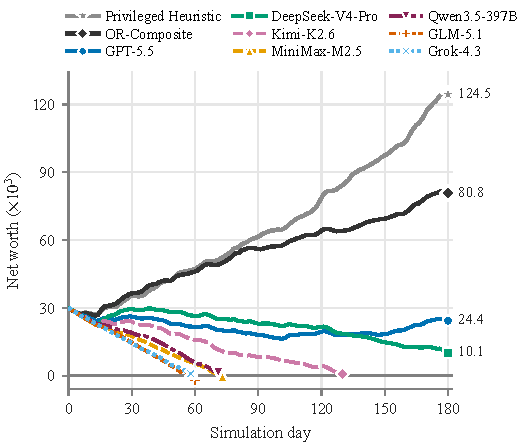
\includegraphics[width=\columnwidth]{figures/net_worth_over_time.pdf}
\caption{Daily net worth trajectories of the two reference
policies and the longest-surviving rollout for each LLM.
Each trajectory terminates when its rollout ends.
Most LLM agents fail to sustain operations over the full
horizon, and even the best-performing agent substantially
underperforms both reference policies in final net worth.
OR-Composite is an operations-research baseline using
only agent-visible information, whereas Oracle is a
privileged reference with access to hidden simulator state.}
\label{fig:net_worth}
\vspace{-2mm}
\end{figure}
% Table 1: comparison with related agent benchmarks (input from introduction.tex so it floats to page 2).
\begin{table*}[t]
\centering
\scriptsize
\setlength{\tabcolsep}{2pt}
\begin{tabular*}{\textwidth}{@{\extracolsep{\fill}}l cc cccc cccc@{}}
\toprule
& \multicolumn{2}{c}{Setting} & \multicolumn{4}{c}{Agent decisions} & \multicolumn{4}{c}{Environment dynamics} \\
\cmidrule(lr){2-3}\cmidrule(lr){4-7}\cmidrule(l){8-11}
Benchmark & Real data & Long-horizon & Pricing & Restock & Supplier & Shelf & Expiry & Reviews & Events & Cash \\
\midrule
WebShop~\citep{3webshopscalablerealworldweb} & \cmark & \xmark & \xmark & \xmark & \xmark & \xmark & \xmark & \pmark & \xmark & \xmark \\
ShoppingBench~\citep{wang2025shoppingbench} & \cmark & \xmark & \xmark & \xmark & \xmark & \xmark & \xmark & \xmark & \xmark & \xmark \\
TheAgentCompany~\citep{xu2024theagentcompany} & \cmark & \pmark & \xmark & \xmark & \xmark & \xmark & \xmark & \xmark & \xmark & \xmark \\
UltraHorizon~\citep{utltabench} & \xmark & \cmark & \xmark & \xmark & \xmark & \xmark & \xmark & \xmark & \xmark & \xmark \\
AIM-Bench~\citep{aimbenchevaluatingdecisionmakingbiases} & \xmark & \pmark & \xmark & \cmark & \pmark & \xmark & \pmark & \xmark & \xmark & \xmark \\
YC-Bench~\citep{he2026ycbench} & \xmark & \cmark & \xmark & \xmark & \xmark & \xmark & \xmark & \xmark & \xmark & \cmark \\
Vending-Bench~\citep{backlund2025vendingbenchbenchmarklongtermcoherence} & \pmark & \cmark & \cmark & \cmark & \cmark & \cmark & \xmark & \xmark & \pmark & \cmark \\
Vending-Bench 2~\citep{andonlabs2025vendingbench2} & \xmark & \cmark & \cmark & \cmark & \cmark & \cmark & \xmark & \pmark & \pmark & \cmark \\
\midrule
\textbf{RetailBench (ours)} & \cmark & \cmark & \cmark & \cmark & \cmark & \cmark & \cmark & \cmark & \cmark & \cmark \\
\bottomrule
\end{tabular*}
\caption{Comparison with related agent benchmarks. Setting: \textbf{Real data} (built on real-world data) and \textbf{Long-horizon} (earlier decisions shape later states over an extended run). Agent decisions: \textbf{Pricing} (set prices), \textbf{Restock} (place replenishment orders), \textbf{Supplier} (choose among suppliers), and \textbf{Shelf} (allocate shelf or slot space). Environment dynamics: \textbf{Expiry} (products expire), \textbf{Reviews} (customer reviews and returns), \textbf{Events} (external demand shocks), and \textbf{Cash} (a cash balance with recurring costs). \cmark{} modeled; \pmark{} partial; \xmark{} absent.}
\label{tab:benchmark_axes}
\vspace{-3mm}
\end{table*}


Large language models (LLMs) with reasoning and tool-use capabilities have made rapid progress on challenging benchmarks for code editing~\citep{swe-bench, tbench_2025}, mathematical and expert-level problem solving~\citep{omni-olpc, hle}, information retrieval~\citep{mialon2023gaiabenchmarkgeneralai, browsecomp}, and web interaction~\citep{webarenarea, mind2web}. However, these benchmark successes often do not translate into equally reliable performance in real-world settings, where agents must sustain coherent decision-making, adapt to evolving conditions, and recover from accumulated errors over extended horizons.

Recent studies reveal substantial limitations in agent reliability in realistic environments, where even leading agents struggle to sustain effective decision-making amid complex operational constraints, evolving conditions, and delayed consequences \citep{kwa2025measuringaiabilitycomplete, metr2025measuring, nof1, andonlabs2025vendingbench2, backlund2025vendingbenchbenchmarklongtermcoherence}. To better capture the complexity of real-world tasks, benchmarks such as OdysseyBench, OSWorld 2.0, EnterpriseOps-Gym, and YC-Bench increasingly evaluate agents in realistic environments involving interconnected decisions, dynamic feedback, and sustained interactions \citep{odysseybenchevaluatingllmagents, yuan2026osworld2,malay2026enterpriseopsgym,he2026ycbench}. However, integrated, data-grounded retail operations remain
underrepresented in existing long-horizon agent evaluations.

To address the limited coverage of integrated, data-grounded
retail operations in existing agent benchmarks, we introduce \textbf{RetailBench}, a controlled, data-grounded benchmark for long-horizon retail operations that captures the complexities of real-world business decision-making. Agents autonomously manage pricing, replenishment, supplier selection, information acquisition, and memory under delivery delays, inventory aging, stockouts, customer feedback, returns, and financial constraints.We evaluate seven LLMs in this realistic retail environment. Figure~\ref{fig:net_worth} reveals substantial gaps in long-horizon operational performance, with only two LLM completing the 180-day horizon. The strongest LLM achieves a final net worth of 24,351 and total sales of 136,405 units, substantially below OR-Composite (80,801 and 202,557), an operations-research reference restricted to agent-visible information (Appendix~\ref{appendix:or_composite}), and the privileged Oracle (124,491 and 263,310). 

To further investigate these performance gaps, we conduct a four-stage analysis of agent trajectories. Our analysis reveals a pronounced disconnect between information acquisition and downstream decision quality: agents demonstrate strong performance in product monitoring and evidence collection, yet struggle to translate acquired evidence into effective decisions and respond promptly to salient operational anomalies amid noisy, high-volume environmental feedback. 
. Our analysis reveals that agents gather evidence effectively but struggle to make high-quality decisions under complex dependencies and respond promptly to operational anomalies. Despite achieving 99.4\% fully evidenced actions, the best-performing agent attains only a 34.8\% high-quality decision rate and a 27.6\% anomaly response rate.

Our main contributions are as follows:

\begin{itemize}[leftmargin=*]
    \item \textbf{A realistic, data-grounded benchmark for long-horizon retail operations.}
    We introduce \textbf{RetailBench}, a controlled, data-grounded environment that captures the complexity of real-world retail operations, where pricing, inventory management, supplier selection, customer feedback, and financial constraints jointly shape long-term outcomes (Section~\ref{sec:env}).

    \item \textbf{Systematic evaluation of agents in realistic, long-horizon settings.}
    We evaluate 19 model--scaffold configurations over a 180-day horizon, revealing substantial limitations in sustained operational performance and large gaps relative to an operations-research reference and a privileged Oracle (Section~\ref{sec:benchmark_results}).

    \item \textbf{Fine-grained diagnosis of long-horizon agent failures.}
    We analyze agent trajectories across four stages: product monitoring, evidence collection, decision-making, and anomaly response. Our findings reveal two recurring failure patterns in realistic operational settings: \textbf{shallow evidence-to-decision integration} and \textbf{limited responsiveness to salient operational anomalies} (Sections~\ref{sec:four_stage_setup} and~\ref{sec:failure_pattern_analysis}).
\end{itemize}

\section{Related Work}
\label{sec:related_work}
\begin{figure*}[t]
\centering
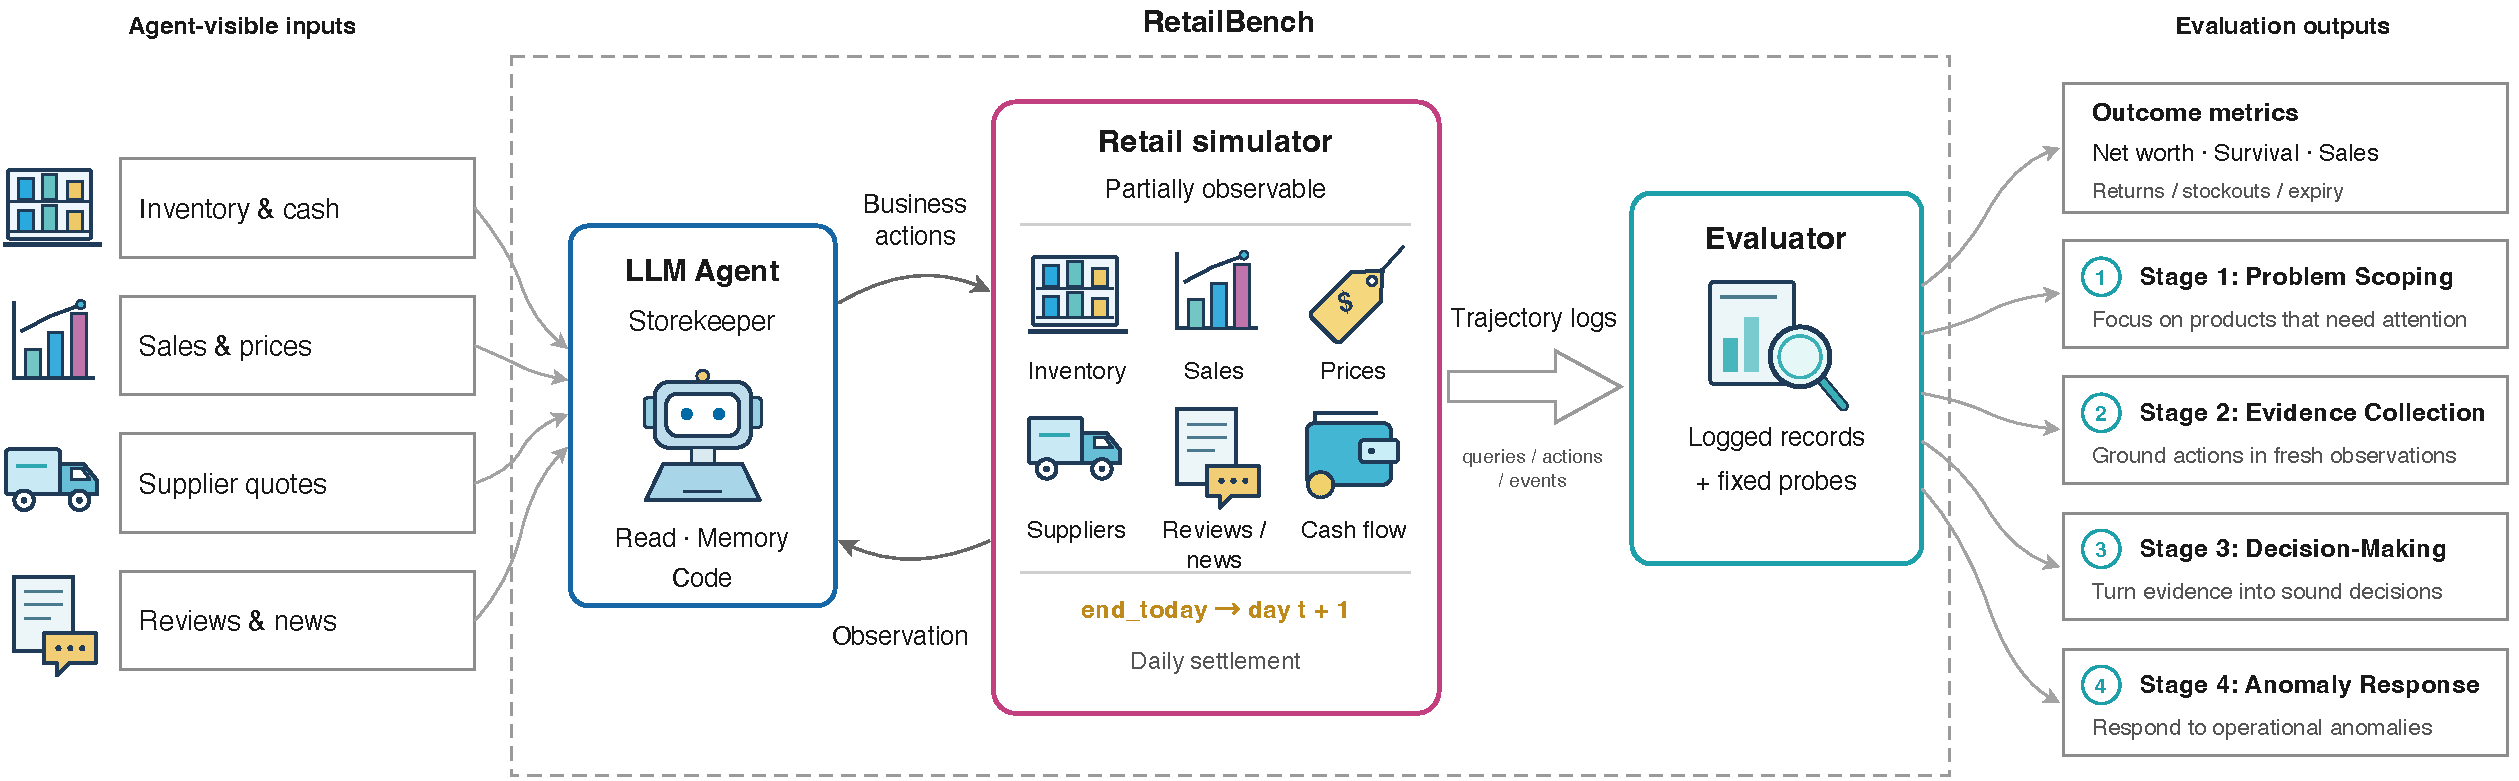
\includegraphics[width=0.96\textwidth]{figures/retailbench_framework.pdf}
\caption{RetailBench interaction framework. A tool-using LLM agent operates a partially observable, data-grounded retail simulator through information queries, auxiliary tools, and business actions. Agent trajectories are evaluated using operational outcomes and four-stage decision diagnostics.}
\label{fig:retailbench_framework}
\vspace{-3mm}
\end{figure*}

\paragraph{Retail, e-commerce, and supply-chain decision benchmarks.}
Prior work has investigated retail and supply-chain decision-making from several complementary perspectives. Retail simulation and promotion optimization study market dynamics and the effects of pricing and promotional strategies~\citep{xia2023retailsynth,xia2024simulationretailpromotions}. Demand recovery and transaction modeling characterize consumer behavior and purchasing patterns using empirical retail data~\citep{wang2025freshretailnet,tkachuk2024consumertransactions}. Web-shopping benchmarks evaluate agents on product search, navigation, and purchasing tasks~\citep{wang2025shoppingbench,3webshopscalablerealworldweb}, while supply-chain and inventory-control studies examine replenishment, resource allocation, and operational decision-making under dynamic constraints~\citep{OFCOURSE,inventory,leluc2023marlimmultiagentreinforcementlearning,invagentlargelanguagemodel,aimbenchevaluatingdecisionmakingbiases}. While these studies address important aspects of retail operations, many focus on individual decision problems rather than integrated, long-horizon business management (Table~\ref{tab:benchmark_axes}). RetailBench complements these efforts with a data-grounded, partially observable supermarket simulator that couples pricing, replenishment, supplier selection, and inventory management over extended horizons.

\paragraph{Long-horizon agent benchmarks.}
Recent benchmarks have extended LLM agent evaluation beyond short-horizon tasks to investigate sustained autonomy, long-term planning, and adaptation in complex environments. These efforts span ultra-long-horizon interactions and office workflows~\citep{utltabench,odysseybenchevaluatingllmagents}, virtual-world planning~\citep{herobenchbenchmarklonghorizonplanning}, lifelong experience reuse~\citep{zheng2025lifelongagentbench}, workplace task execution~\citep{xu2024theagentcompany}, and sustained business operations~\citep{backlund2025vendingbenchbenchmarklongtermcoherence,andonlabs2025vendingbench2}. Collectively, they examine complementary aspects of long-term agent behavior, including sequential planning, experience accumulation, and reliable execution over extended interactions. RetailBench complements these efforts by introducing a data-grounded, closed-loop benchmark for evaluating long-horizon agent performance in realistic business operations.


\section{Environment Construction}
\label{sec:env}


\subsection{Interface}

RetailBench models single-store supermarket operations as a partially
observable decision process over 180 simulated days. Agents manage
pricing, replenishment, and supplier selection through tool-based
interactions, as illustrated in Figure~\ref{fig:retailbench_framework}.
These decisions are interdependent and have delayed consequences:
pricing and replenishment affect future sales and inventory, while
delivery delays, product expiration, and market changes influence
subsequent operations and financial outcomes.

Formally, we model RetailBench as a partially observable Markov
decision process (POMDP):
\begin{equation}
\label{eq:pomdp}
\mathcal{M} = (\mathcal{S}, \mathcal{A}, \mathcal{O}, T, \Omega, R),
\end{equation}
where $\mathcal{S}$ is the state space, $\mathcal{A}$ the tool-action
space, $\mathcal{O}$ the observation space, $T$ the transition function,
$\Omega$ the observation function, and $R$ the business-outcome
function. Agents observe the environment only through available tools,
without access to its full underlying state. Appendix~\ref{app:state_action_spaces}
provides the detailed state and action spaces.

At day $t$ and intra-day step $k$, the environment state is
factorized as:
\begin{equation}
\label{eq:latent_state}
S_{t,k} = (P, I, V, C, D, E, F)_{t,k},
\end{equation}
where $P$ denotes product attributes and prices, $I$ inventory and
pending orders, $V$ shelf assortment, $C$ supplier conditions,
$D$ demand factors, $E$ external events, and $F$ financial state.
These components jointly characterize retail operations under
inventory, shelf-capacity, and financial constraints.

Agents interact with RetailBench through three categories of tools:
read-only tools for information acquisition,
auxiliary tools for memory and computation, and
operational tools for business decisions.
At day $t$ and interaction step $k$, let $S_{t,k}$ denote the
environment state, $h_{t,k}$ the agent's interaction history,
and $a_{t,k}$ the selected tool action.
The interaction is formalized as
\begin{equation}
\label{eq:agent_interaction}
\begin{aligned}
\mathcal{A} &=
\mathcal{A}^{\mathrm{read}}
\cup \mathcal{A}^{\mathrm{other}}
\cup \mathcal{A}^{\mathrm{act}},\\
o_{t,k} &= \Omega(S_{t,k},a_{t,k}),
\, a_{t,k}\in\mathcal{A}^{\mathrm{read}},\\
z_{t,k} &= G(h_{t,k},a_{t,k}),
\, a_{t,k}\in\mathcal{A}^{\mathrm{other}},\\
S_{t,k+1} &= T(S_{t,k},a_{t,k}),
\, a_{t,k}\in
\mathcal{A}^{\mathrm{act}}\!\setminus\!\{a^{\mathrm{end}}\}.
\end{aligned}
\end{equation}

Here, $\Omega$ is the observation function that returns
environment information $o_{t,k}$, while $G$ represents
auxiliary operations producing outputs $z_{t,k}$ from
the agent's interaction history.
The transition function $T$ updates the environment state
following operational actions, whereas read-only and
auxiliary tools leave the simulator state unchanged.
Specifically, read-only tools expose inventory, sales,
supplier quotes, and customer feedback without revealing
latent demand or supplier-quality parameters.
Auxiliary tools support memory and computation, while
operational tools enable pricing, replenishment,
shelf management, and persistent note updates.

Time advances only when the agent invokes \texttt{end\_today},
which triggers the daily settlement:
\begin{equation}
\label{eq:end_today_transition}
S_{t+1,0}
= T(S_{t,k},a^{\mathrm{end}})
\equiv T_{\mathrm{day}}(S_{t,k}).
\end{equation}
This transition processes deliveries, sales, customer feedback,
returns, product expiration, operating costs, and market changes.
Consequently, current decisions shape future inventory, cash flow,
and operational opportunities, requiring agents to balance
short-term performance with long-term profitability and survival.

\subsection{Data-Grounded Simulator}

RetailBench integrates real-world retail data with controlled simulation
mechanisms to model long-horizon business operations. Its data sources
provide empirical foundations for retail demand, pricing, customer
feedback, and external events.

We use the Dominick's dataset~\citep{DominicksDataset}, which contains
store-level records of product categories, sales, prices, and
cost-related information. These records inform the product catalog
and empirical priors for demand, store traffic, pricing, and
procurement costs. We select 96 products across 20 categories
with sufficient records to estimate product-level demand and
category-level substitution patterns.

Customer feedback is grounded in Amazon Reviews
2023~\citep{hou2024bridging}, which provides category-specific review
pools organized by ratings, sentiment, and product aspects.
Realized sales generate reviews whose ratings depend on supplier
quality, with comments sampled from the corresponding generated reviews pool.
External events are constructed from financial news
articles~\citep{ashraq2025financialNewsArticles}, covering neutral,
category-level, and product-level events.
Agents observe news and historical feedback, while latent event
parameters govern their effects on demand and supply.

Together, these sources provide data-grounded operational signals
within a controlled, partially observable simulation environment.


\subsection{Modules}
\label{sec:module_logic}

RetailBench comprises seven interconnected modules: Inventory,
Suppliers \& Orders, Shelf, Customer Demand, Reviews \& Returns,
News Events, and Finance \& Records
(Appendix~\ref{app:simulator_modules}).
Together, these modules govern inventory availability, supplier
conditions, demand realization, customer feedback, external events,
and financial outcomes.

Module interactions introduce dependencies across operational decisions
and time. Replenishment affects future inventory through delivery
delays, while pricing and shelf allocation influence realized sales.
Inventory aging, returns, and operating costs further affect
subsequent inventory availability and financial conditions.
Consequently, operational decisions have delayed effects that
shape future states and constrain subsequent actions.

Detailed module definitions and day-level update equations are
provided in Appendix~\ref{app:simulator_modules}
and Appendix~\ref{app:simulator_update_equations}.


\subsection{Scope}

RetailBench focuses on integrated, single-store retail operations
rather than isolated operational subproblems
(Section~\ref{sec:related_work}; Table~\ref{tab:benchmark_axes}).
By integrating data-grounded business conditions, interdependent decisions, and delayed consequences, RetailBench provides a controlled yet realistic retail environment for evaluating long-horizon agent decision-making under partial observability.

\section{Experimental Setup}
\label{sec:evaluation_protocol}
\subsection{Environment Configuration}

All evaluations use a fixed RetailBench configuration designed to capture the complexity of sustained retail operations. The environment comprises 96 products across 20 categories, with five candidate suppliers per product whose price--quality profiles evolve over time. Customer reviews and daily news events introduce additional operational feedback. Agents operate with an initial budget of 30{,}000, daily rent of 600, an inventory capacity of 15{,}000 units, and a shelf capacity of 40 products. Each rollout spans up to 180 days and terminates upon bankruptcy,
defined as five consecutive days of negative funds. Complete environment settings are provided in Appendix~\ref{appendix:env_setting}.


\subsection{Models and Scaffolds}
\label{sec:models_frameworks}

We evaluate LLM agents using three prompting-based scaffolds: ReAct~\citep{yao2023react}, Reflection~\citep{reflection}, and Plan-and-Act~\citep{erdogan2025planandactimprovingplanningagents}. These scaffolds represent common agent interaction patterns and operate through the same RetailBench tool interface; Appendix~\ref{appendix:prompts} lists their prompts.

Our evaluation covers seven LLMs and 19 model--scaffold configurations: six models under all three scaffolds and GPT-5.5 under ReAct only. For models with complete scaffold coverage, we report means and sample standard deviations across scaffolds, reflecting scaffold sensitivity rather than seed-level uncertainty. 


\subsection{Reference Policies}
\label{sec:references}

We compare LLM agents against two non-LLM reference policies that differ in information access: OR-Composite uses only agent-visible information, whereas the Privileged Heuristic reads hidden simulator state.

\paragraph{OR-Composite.}
OR-Composite is a classical operations-research reference restricted to agent-visible information. It combines textbook rules for four decisions: a fixed assortment of at most two SKUs per category ranked by visible historical contribution; quality-first supplier selection~\citep{dickson1966vendor,weber1991vendor} that ranks vendors by an upper confidence bound on observed return rates~\citep{brown2001interval}; daily-review $(s,S)$ replenishment capped by shelf life~\citep{silver2017inventory,nahmias1982perishable}; and weekly constant-elasticity markup pricing over return-adjusted costs~\citep{phillips2021pricing}. It never reads latent supplier quality, hidden demand, news effects, or future outcomes. Appendix~\ref{appendix:or_composite} gives the full specification, parameters, and information-access audit.

\paragraph{Privileged Heuristic.}
The Privileged Heuristic is a hand-specified, rule-based reference with access to hidden simulator state. It reads structured simulator state that agents cannot observe, including supplier quality scores and news impact values: it orders each product from its highest-quality supplier, sets prices that maximize historical profit, and scales replenishment to news-adjusted demand targets. It is neither a fair baseline for LLM agents nor an upper bound, because it follows a fixed hand-specified rule and faces none of the agents' prompt, tool-selection, or memory constraints. Appendix~\ref{appendix:handcrafted_policy} gives its algorithm and parameter settings.

% Table 2 is defined here so that it floats to the top of page 6.
\begin{table*}[t]
\centering
\footnotesize
\setlength{\tabcolsep}{3.0pt}
\renewcommand{\arraystretch}{1.08}
\resizebox{\textwidth}{!}{%
\begin{tabular}{lrrrrrrr}
\toprule
Entry & Days $\uparrow$ & Net worth $\uparrow$ & Sales $\uparrow$ & Return $\downarrow$ & Expired $\downarrow$ & Stockout-day rate $\downarrow$ & Tokens per Day $\downarrow$ \\
\midrule
DeepSeek-V4-Pro & \secondval{139.3 $\pm$ 43.2} & 2,258.10 $\pm$ 6,810.42 & \secondval{110,980 $\pm$ 68,622} & \secondval{0.094 $\pm$ 0.007} & 0.039 $\pm$ 0.022 & 0.659 $\pm$ 0.111 & 450,693 $\pm$ 62,795 \\
GLM-5.1 & 55.0 $\pm$ 5.6 & -113.13 $\pm$ 4,113.31 & 4,842 $\pm$ 3,555 & \secondval{0.094 $\pm$ 0.053} & 0.013 $\pm$ 0.015 & \bestval{0.300 $\pm$ 0.148} & 1,016,126 $\pm$ 157,931 \\
Grok-4.3 & 40.3 $\pm$ 24.8 & \secondval{8,201.74 $\pm$ 12,806.30} & 10,861 $\pm$ 10,275 & 0.095 $\pm$ 0.038 & 0.077 $\pm$ 0.088 & \secondval{0.395 $\pm$ 0.036} & \secondval{259,191 $\pm$ 171,982} \\
Kimi-K2.6 & 95.0 $\pm$ 32.4 & 1,566.00 $\pm$ 4,005.87 & 55,317 $\pm$ 28,258 & 0.109 $\pm$ 0.016 & 0.014 $\pm$ 0.023 & 0.533 $\pm$ 0.103 & 684,782 $\pm$ 295,717 \\
MiniMax-M2.5 & 63.3 $\pm$ 8.7 & 602.42 $\pm$ 1,104.83 & 20,908 $\pm$ 3,587 & 0.105 $\pm$ 0.002 & \bestval{0.005 $\pm$ 0.003} & 0.731 $\pm$ 0.081 & 802,006 $\pm$ 419,031 \\
Qwen3.5-397B-A17B & 57.0 $\pm$ 12.1 & 3,709.77 $\pm$ 2,473.06 & 32,857 $\pm$ 2,774 & 0.106 $\pm$ 0.010 & 0.069 $\pm$ 0.036 & 0.645 $\pm$ 0.057 & 886,581 $\pm$ 179,962 \\
GPT-5.5 & \bestval{180.0 $\pm$ --} & \bestval{24,350.98 $\pm$ --} & \bestval{136,405 $\pm$ --} & \bestval{0.065 $\pm$ --} & \secondval{0.011 $\pm$ --} & 0.761 $\pm$ -- & \bestval{176,260 $\pm$ --} \\
\midrule
OR-Composite (classical OR) & 180.0 & 80,801.21 & 202,557 & 0.047 & 0.013 & 0.417 & \\
\midrule
Oracle Policy & 180.0 & 124,491.15 & 263,310 & 0.020 & 0.024 & 0.678 & \\
\bottomrule
\end{tabular}
}
\caption{Model-level outcome summary.
Results are reported as mean $\pm$ sample standard deviation
across three scaffolds, except GPT-5.5 (ReAct only).
LLM agents substantially underperform both references,
with the best LLM achieving only 30.1\% of OR-Composite's
final net worth.
Bold and underline indicate the best and second-best LLM results.
OR-Composite uses only agent-visible information
(Appendix~\ref{appendix:or_composite}),
while Oracle is a privileged reference
(Appendix~\ref{appendix:oracle}).}
\label{tab:aggregate_main_results}
\vspace{-3mm}
\end{table*}


\subsection{Outcome and Resource Metrics}

We evaluate long-horizon operational performance through three categories of business outcomes and two categories of resource diagnostics. Arrows indicate the preferred direction for outcome metrics.

\begin{itemize}[leftmargin=*]

    \item \textbf{Operational viability.}
    \textbf{Final Net Worth} ($\uparrow$) measures terminal asset value, including cash, on-hand inventory, and pending-order value. \textbf{Survival Days} ($\uparrow$) measures the duration of continued store operation.

    \item \textbf{Sales effectiveness.}
    \textbf{Final Total Sales} ($\uparrow$) measures cumulative units sold; and \textbf{Return Ratio} ($\downarrow$) measures the fraction of sold units that are returned.

    \item \textbf{Inventory control.}
    \textbf{Stockout Days} ($\downarrow$) counts days on which at least one product has insufficient inventory, while \textbf{Expired Ratio} ($\downarrow$) measures the fraction of expired units among all units sold or expired.

    \item \textbf{Token use.}
    \textbf{Tokens per Day} measures average token consumption as a resource-efficiency diagnostic.

\end{itemize}


\subsection{Four-Stage Diagnosis}
\label{sec:four_stage_setup}

Outcome metrics quantify long-horizon operational performance but provide limited insight into where agent decision-making breaks down. To investigate these limitations, we introduce a four-stage trajectory analysis covering product monitoring, evidence collection, decision-making, and anomaly response. Each stage is evaluated using an auditable, trace-based metric that captures a distinct aspect of operational behavior.

\begin{itemize}[leftmargin=*]

    \item \textbf{Stage 1: Product Monitoring.}
    Measures product-level inspection coverage as the fraction of products sold on day $t-1$ that receive a successful product-specific query on day $t$. Store-wide listings are excluded.

    \item \textbf{Stage 2: Evidence Collection.}
    Measures evidence completeness as the fraction of executed orders and price updates for which all required evidence dimensions were observed within their category-specific validity windows.

    \item \textbf{Stage 3: Decision-Making.}
    Measures decision-making ability in order sizing and supplier selection by averaging two shares computed from simulator state on the action day. The order-quantity share is the fraction of order lines whose post-arrival days of cover fall between the selected supplier’s maximum quoted lead time and the product’s shelf life. Days of cover are calculated by dividing the sum of inventory position and ordered quantity by expected daily demand at the agent’s current price. The supplier-quality share is the fraction of order lines assigned to the highest-quality supplier among the five candidates. These evaluator-side measures characterize ordering decisions but do not establish overall decision optimality, which also depends on pricing.
 
    
    \item \textbf{Stage 4: Anomaly Response.}
    Measures operational response coverage as the fraction of stockout and expiration events followed by an executed order or price adjustment for the affected product within three days. Events whose three-day windows extend beyond the last completed day are right-censored and excluded.

\end{itemize}

The four metrics are evaluated independently and Appendix~\ref{appendix:stage_metrics} provides the complete metric definitions, denominators, censoring rules, and finer per-stage analyses.

\section{Results}
\label{sec:experiment}
\subsection{Experimental Results}
\label{sec:benchmark_results}
\label{sec:failure_pattern_analysis}
\label{sec:failure_analysis}

% Figure 3 is defined here so that it floats to the top of page 7.
\begin{figure*}[t]
    \centering
    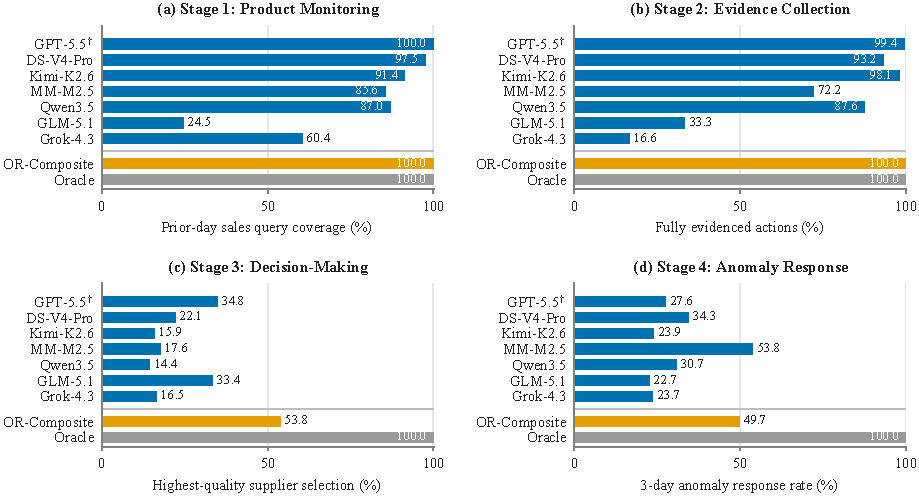
\includegraphics[width=\textwidth]{figures/four_stage_scores.pdf}
   \caption{Model-level outcome summary.
Results are reported as mean $\pm$ sample standard deviation
across three scaffolds, except GPT-5.5 (ReAct only).
LLM agents substantially underperform both references,
with the best LLM achieving only 30.1\% of OR-Composite's
final net worth.
Bold and underline indicate the best and second-best LLM results.
OR-Composite uses only agent-visible information
(Appendix~\ref{appendix:or_composite}),
while Oracle is a privileged reference
(Appendix~\ref{appendix:handcrafted_policy}).}
    \label{fig:four_stage_scores}
    \vspace{-2mm}
\end{figure*}

\paragraph{Long-horizon operational performance.}
Table~\ref{tab:aggregate_main_results} summarizes performance across ReAct, Reflection, and Plan-and-Act for the six models with complete scaffold coverage, reporting means and sample standard deviations across scaffolds rather than independent trials. GPT-5.5 is evaluated under ReAct only. No scaffold consistently dominates, with ReAct, Reflection, and Plan-and-Act achieving win counts of 2/2/2 for both final net worth and sales, and 3/1/2 for survival. Results for all 19 rollouts and the scaffold win counts are provided in Appendix~\ref{appendix:rollout_results}.

Results reveal substantial limitations in sustaining effective operations over long horizons. Mean survival ranges from 40.3 days (Grok-4.3) to 139.3 days (DeepSeek-V4-Pro), with none of the six fully evaluated models reaching the 180-day horizon on average. Only two of 19 rollouts complete all 180 days: DeepSeek-V4-Pro with Plan-and-Act and GPT-5.5 with ReAct. Moreover, completing the horizon does not guarantee strong business performance. The privileged Oracle achieves a final net worth of 124{,}491.15 and sales of 263{,}310 units, compared with 80{,}801.21 and 202{,}557 units for OR-Composite. DeepSeek-V4-Pro achieves the highest across-scaffold mean sales among fully evaluated models (110{,}980 units), while GPT-5.5 (ReAct), despite completing the full horizon, achieves only 24{,}350.98 in final net worth and 136{,}405 units in sales. These results reveal a substantial gap between sustained operation and effective long-horizon business performance.

\paragraph{Four-stage decision-making diagnosis.}
To examine where these performance gaps arise, we analyze agent trajectories across four stages: product monitoring, evidence collection, decision-making, and anomaly response (Section~\ref{sec:four_stage_setup}). Figure~\ref{fig:four_stage_scores} reports the corresponding diagnostic scores, with LLM results averaged over evaluated scaffolds. We additionally report pooled statistics across all 19 rollouts and individual-rollout ranges. These analyses are descriptive, with one rollout per model--scaffold configuration. Detailed breakdowns are provided in Appendix~\ref{appendix:stage_metrics}.

\paragraph{Four-stage decision-making diagnosis.}
To characterize the observed performance gaps, we analyze agent
trajectories across four stages: product monitoring, evidence collection,
decision-making, and anomaly response
(Section~\ref{sec:four_stage_setup}).
Figure~\ref{fig:four_stage_scores} summarizes the corresponding
diagnostic scores across models and reference policies.
A general pattern emerges: LLM agents perform relatively well
in product monitoring and evidence collection, but show substantially
weaker performance in decision-making and anomaly response.
We further examine these patterns using pooled statistics from
all 19 rollouts and individual-rollout results.
These analyses are descriptive, with one rollout per
model--scaffold configuration. Detailed results are provided
in Appendix~\ref{appendix:stage_metrics}.

\paragraph{Product Monitoring and evidence collection: effective information acquisition.}
As shown in Figure~\ref{fig:four_stage_scores}, most models
perform relatively well in the first two stages.
Across all LLM rollouts, 91.8\% of 31{,}527 sold
product--days receive a product-specific query on the following
day. Five of seven models achieve mean Stage~1 scores above
85\%, while GPT-5.5, DeepSeek-V4-Pro, and Kimi-K2.6 exceed
93\% in Stage~2. In contrast, GLM-5.1 and Grok-4.3 exhibit
substantially lower scores, particularly in evidence collection
(33.3\% and 16.6\%, respectively).
These results suggest that information acquisition is
relatively reliable among stronger agents, although
substantial variation remains across models.

\paragraph{Decision-making: shallow evidence-to-decision integration.}
Despite relatively strong evidence collection,
Figure~\ref{fig:four_stage_scores} reveals a pronounced
decline in supplier decision-making scores.
Across 5{,}172 order lines, LLM agents select the
highest-quality supplier in only 21.6\% of cases,
close to the 20\% random-choice baseline.
Model-level means range from 14.4\% to 34.8\%,
compared with 53.8\% for OR-Composite.
Although GLM-5.1 with Plan-and-Act achieves 56.0\%,
this result is based on only 50 orders.
As agents observe noisy quality signals and must balance
supplier quality against price, this metric does not
directly measure business decision optimality.
Nevertheless, considered alongside their weaker overall
business outcomes, these findings suggest
\textbf{shallow evidence-to-decision integration}:
agents struggle to translate acquired information
into economically effective decisions.

\paragraph{Anomaly response: inconsistent operational follow-up.}
Figure~\ref{fig:four_stage_scores} further shows limited
responsiveness to operational anomalies.
Among 2{,}374 eligible stockout and expiration events,
only 33.7\% are followed by an order or price adjustment
within three days, with response rates of 35.0\% for
stockouts and 22.8\% for expirations.
An additional 86 events are right-censored.
Model-level response rates range from 22.7\% to 53.8\%,
with no individual rollout exceeding 57.0\%.
Importantly, response frequency does not necessarily
reflect corrective effectiveness: OR-Composite achieves
a lower response rate than MiniMax-M2.5
(49.7\% vs. 53.8\%), yet substantially higher final
net worth (80{,}801.21 vs. 602.42).
Stage~4 therefore measures response coverage rather than
corrective effectiveness, revealing
\textbf{inconsistent operational follow-up}
among LLM agents.


\paragraph{Summary.}
Together, the outcome and trajectory analyses highlight persistent
challenges in long-horizon retail operations. Despite relatively
strong performance in product monitoring and evidence collection,
LLM agents exhibit near-chance supplier-quality selection, while
approximately two-thirds of eligible operational anomalies receive
no corresponding action within three days. These findings reveal
two recurring failure patterns:
\textbf{shallow evidence-to-decision integration} and
\textbf{limited responsiveness to salient operational anomalies},
which may partly explain the poor long-horizon performance
observed in some agents.

\section{Conclusion}
\label{sec:conclusion}
We introduced \textbf{RetailBench}, a data-grounded benchmark for evaluating long-horizon decision-making by tool-using LLM agents in realistic retail environments. By integrating interdependent business decisions, dynamic feedback, and delayed consequences, RetailBench captures key complexities of real-world retail operations within a controlled evaluation setting.

Across seven LLMs and 19 model--scaffold configurations, our results reveal substantial challenges in sustaining effective decision-making over extended horizons. Only two rollouts complete the 180-day horizon, and even the best-performing agent substantially underperforms the OR-Composite and Privileged Heuristic references. Our four-stage trajectory analysis further reveals a gap between information acquisition and decision quality: agents often gather relevant evidence but exhibit \textbf{shallow evidence-to-decision integration} and \textbf{limited responsiveness to salient operational anomalies}.
These findings establish RetailBench as a testbed for evaluating and diagnosing long-horizon agent capabilities in realistic economic environments, highlighting the challenges of maintaining coherent and adaptive decision-making under complex operational constraints.

\noindent\textbf{Code and data availability.}
Our \href{https://anonymous.4open.science/r/RetailBench_ARR-6253}{code}, benchmark materials, processed data, and reproduction instructions are publicly available.


\section{Limitations}
\label{sec:limitation}
RetailBench is designed as a controlled, data-grounded benchmark for evaluating long-horizon decision-making rather than a comprehensive simulation of retail operations. Its current implementation focuses on single-store operations, combining real-world retail data with simulated dynamics to capture interdependent decisions and delayed consequences. Extending the environment to multi-store and multi-agent settings could further broaden its applicability.

Our evaluation covers seven LLMs across 19 prompting-based model--scaffold configurations under a fixed environment setting. As each configuration contains a single rollout, the reported across-scaffold statistics characterize variation across scaffolds rather than seed-level uncertainty. Furthermore, the four-stage trajectory analysis provides descriptive insights into agent behavior without establishing causal relationships between individual decision patterns and operational outcomes.

Future work could explore more diverse environment configurations, repeated evaluations, and advanced stateful or learning-based agents to further investigate long-horizon robustness and adaptation.

% Bibliography entries for the entire Anthology, followed by custom entries
%\bibliography{anthology,custom}
% Custom bibliography entries only
\bibliography{custom}

\appendix
\section{Simulator}
\label{appendix:simulator}

\subsection{Simulator Modules}
\label{app:simulator_modules}

RetailBench follows a seven-module organization: Inventory, Suppliers \& Orders, Shelf, Customer Demand, Reviews \& Returns, News Events, and Finance \& Records. Static product attributes, including identity, category, shelf life, retail price, historical sales summaries, and review summaries, are shared across these modules. The modules are coupled through the daily transition process: orders create delayed deliveries, shelf-assortment decisions determine customer-facing availability, demand is realized as sales, reviews and returns update feedback signals, news changes demand or supply conditions, and finance records cash-flow outcomes and store viability.

\paragraph{Inventory.}
The inventory module tracks physical stock state, including on-hand units, item age, sellable quantity, capacity constraints, stockouts, expirations, and waiting items that cannot yet enter inventory because of capacity limits. It determines the feasibility constraints for procurement, shelving, and sales.

\paragraph{Shelf.}
The shelf module enforces a finite shelf capacity and determines the customer-facing assortment. Stocked products that are not on the shelf remain in inventory but are not visible to customers and therefore cannot generate demand.

\paragraph{Suppliers \& Orders.}
The suppliers-and-orders module provides five procurement candidates per product, each with cost, quality, and delivery-time profiles. Supplier choices affect procurement expenditure, delivery timing, return risk, reviews, and future inventory availability. Replenishment orders are converted into delayed deliveries that enter inventory on later days when capacity allows.

\paragraph{Customer Demand.}
Following RetailSynth~\citep{xia2023retailsynth}, customer choice follows an MNL model~\citep{mcfadden_conditional_1974}. Daily traffic comes from Dominick's~\citep{DominicksDataset}. The simulator first samples category demand from power-aggregated shelf-visible attraction~\citep{nakanishi1974mci}, then allocates it across visible products. The corresponding update equations are given in Appendix~\ref{app:simulator_update_equations}.

\paragraph{Reviews \& Returns.}
The reviews-and-returns module converts realized sales and supplier quality into post-sale feedback. Sold items can generate product-level reviews, which update rating summaries and later demand through $\rho^{\mathrm{rev}}_{jt}$. Returned units are sampled from supplier-quality-dependent return probabilities, logged at the product and supplier level, and deducted from realized revenue. Thus, supplier quality affects both customer feedback and return pressure.

\paragraph{News Events.}
The news-events module samples observable news text with hidden simulator metadata specifying impact scope, target category or product, direction, strength, affected side, and duration. Demand-side news changes product attraction through $\rho^{\mathrm{news}}_{jt}$, while supply-side news changes supplier costs through $\delta^{\mathrm{sup}}_{jt}$.

\paragraph{Finance \& Records.}
The finance-and-records module tracks revenue, procurement cost, returns, rent, cash, inventory value, pending-order value, net worth, and persistent sales, supplier, review, return, and news records. At each day transition, the simulator applies deliveries, shelf-constrained demand realization, sales, feedback updates, expiration, rent, cash-flow updates, and next-day supplier/news changes.

\subsection{State and Action Spaces}
\label{app:state_action_spaces}

We construct the environment using real-world retail data from the Dominick’s dataset \citep{DominicksDataset}. From the 20 available product categories, we select 96 products with the most complete and informative sales records. The richness of these observations enables reliable modeling of the relationship between pricing decisions and realized demand. The same source provides the cost priors and the historical sales records used to calibrate the demand model.

\paragraph{Key Symbols.}
Let $\mathcal{J}$ denote the set of selected products, with cardinality $|\mathcal{J}| = J$ (where $J=96$ in our experiments). Each product $j \in \mathcal{J}$ belongs to a product category $\mathrm{cat}(j) \in \{1,\ldots,20\}$. For each product $j$, let $\mathcal{K}(j)$ denote its associated supplier set, with $|\mathcal{K}(j)| = 5$. Let $V_t\subseteq\mathcal{J}$ denote the product set placed on shelf on day $t$.

\paragraph{State and action spaces.}
The simulator state space is $\mathcal{S}=\mathcal{S}^{\mathrm{prod}}\times\mathcal{S}^{\mathrm{inv}}\times\mathcal{S}^{\mathrm{shelf}}\times\mathcal{S}^{\mathrm{sup}}\times\mathcal{S}^{\mathrm{dem}}\times\mathcal{S}^{\mathrm{ext}}\times\mathcal{S}^{\mathrm{fin}}$, covering product attributes and prices, inventory and pending deliveries, shelf assortment, supplier candidates, demand signals, external news, and financial accounting. The action space is $\mathcal{A}=\mathcal{A}^{\mathrm{read}}\cup\mathcal{A}^{\mathrm{other}}\cup\mathcal{A}^{\mathrm{act}}$, which contains read-only observation tools, constrained analysis tools, and state-changing tools; Appendix~\ref{app:action_space_details} lists every tool.

\subsubsection{Product State \texorpdfstring{$S_t^{\text{prod}}$}{S t prod}}

For each product $j$, we maintain a set of static attributes together with time-varying operational signals:
\begin{equation}
S_{t,j}^{\text{prod}} =
\big(
\texttt{id}_j,\ \texttt{desc}_j,\ L_j,\ p_{jt},\ \mathbf{h}^{\text{sales}}_{j,t},\ \mathbf{r}_{j,t}
\big).
\end{equation}
Here, $\texttt{id}_j$ and $\texttt{desc}_j$ denote the unique identifier and textual description of product $j$, respectively. $L_j$ denotes the shelf life (in days), and $p_{jt}$ is the retail price on day $t$. The term $\mathbf{h}^{\text{sales}}_{j,t}$ encodes historical sales statistics, while $\mathbf{r}_{j,t}$ summarizes aggregated customer review signals, such as average rating and review volume.

\subsubsection{Inventory and Shelf State \texorpdfstring{$S_t^{\text{inv}}$, $S_t^{\text{shelf}}$}{S t inv, S t shelf}}

Inventory is represented at the product level with age tracking. Let $I_{jt}$ denote the on-hand units of product $j$ at the beginning of day $t$. To support shelf-life constraints and depreciation, we track the arrival time and remaining shelf life of each unit.

\paragraph{Capacity constraint and pending queue.}
Let $\mathrm{Cap}$ denote the total inventory capacity of the store. If incoming replenishment orders would violate this constraint, excess units are placed into a first-in-first-out (FIFO) pending queue $\mathcal{Q}_t$ and become available only after sufficient inventory space is released:
\begin{equation}
\sum_{j\in\mathcal{J}} \sum_{a=0}^{L_j} I_{jt}^{(a)} \le \mathrm{Cap}.
\end{equation}

\paragraph{Stockout signal.}
When realized demand exceeds the available sellable inventory of product $j$ on day $t$, a stockout indicator is triggered. This signal is recorded at the end of day $t$ and exposed to the agent as explicit operational feedback.

\paragraph{Expiration and destruction.}
At each day transition, inventory units whose residence time exceeds their shelf life are removed from the system.

\paragraph{Shelf assortment.}
The active shelf assortment $V_t$ has finite product capacity:
\begin{equation}
V_t \subseteq \mathcal{J}, \qquad |V_t| \le C^{\mathrm{shelf}}.
\end{equation}
Only products in $V_t$ are visible to customer demand; newly delivered inventory remains off shelf until the agent updates $V_t$ through the shelf-assortment action.

\subsubsection{Supply Chain State \texorpdfstring{$S_t^{\text{sup}}$}{S t sup}}

Each product $j$ is associated with a set of suppliers $k \in \mathcal{K}(j)$. The supplier state includes procurement price $c_{jk}$, quality level $q_{jk}$, and delivery-time distribution:
\begin{equation}
S_{t,j}^{\text{sup}} =
\big\{(c_{jk}, q_{jk}, \mathcal{L}_{jk}) : k \in \mathcal{K}(j)\big\}.
\end{equation}
Delivery time $\ell_{jk} \sim \mathcal{L}_{jk}$ is sampled when an order is placed. Procurement prices are discretized into tiers using Dominick’s cost signals \citep{DominicksDataset}; mapping higher price tiers to higher quality levels is a modeling assumption, motivated by the positive price--quality correlations reported for national brands and non-food private labels \citep{supplychain}.

\paragraph{Enforced diversity.}
To avoid degenerate supplier configurations, we enforce that each product has (i) one supplier with maximal quality, (ii) one supplier with minimal price and minimal quality, and remaining suppliers spanning intermediate price–quality levels.

\subsubsection{Demand Signals \texorpdfstring{$S_t^{\text{dem}}$}{S t dem}}
\label{app:demand}

Demand-related components capture customer traffic, shelf-visible choice sets, and stochastic sales generation. We define
\begin{equation}
S_t^{\text{dem}} =
\big(
N_t,\ \{A^0_{jt},\rho^{\mathrm{rev}}_{jt},\rho^{\mathrm{news}}_{jt}\}_{j\in\mathcal{J}}
\big),
\end{equation}
where $N_t$ denotes daily customer traffic derived from the Dominick’s dataset, $A^0_{jt}$ is the calibrated base attraction, and $\rho^{\mathrm{rev}}_{jt}$ and $\rho^{\mathrm{news}}_{jt}$ are bounded demand-side effects from reviews and news. Given traffic $N_t$, prices $\{p_{jt}\}_{j\in\mathcal{J}}$, shelf assortment $V_t$, review signals, and active news, realized sales follow Equations~\ref{eq:base_attraction}--\ref{eq:demand_sales}; a product $j\notin V_t$ receives no demand on that day.

\subsubsection{External Information \texorpdfstring{$S_t^{\text{ext}}$}{S t ext}}

We maintain a set of active news events $\mathcal{E}_t$. Each event $e \in \mathcal{E}_t$ is stored as
\begin{equation}
e=(m,\tau,\texttt{side},\texttt{sign},s,\texttt{text},\texttt{ttl}),
\label{eq:news_record}
\end{equation}
where $m \in \{\text{neutral}, \text{macro}, \text{category}, \text{product}\}$ is the event mode (impact scope), $\tau$ is the targeted category or product, \texttt{side} $\in \{\text{demand}, \text{supply}, \text{both}\}$ is the affected side, \texttt{sign} $\in \{+1,-1\}$ is the impact direction, $s$ is the impact strength, \texttt{text} is the observable news content, and \texttt{ttl} is the number of days the event remains active. Neutral news has $s = 0$ by design. News texts are grounded in financial-news-articles~\citep{ashraq2025financialNewsArticles} and expanded into retail-relevant events through LLM-assisted rewriting and metadata annotation. Depending on \texttt{side} and $m$, an event changes demand attraction, supplier prices, or both (Appendix~\ref{app:simulator_update_equations}).

\subsubsection{Simulator Update Equations}
\label{app:simulator_update_equations}

This section gives the detailed equations summarized in Section~\ref{sec:module_logic}.

\paragraph{Supply price update.}
Let $\bar c_{jkt}$ be the base procurement price for supplier $k$ and product $j$ on day $t$, and let $\delta^{\mathrm{sup}}_{jt}$ be the active supply-side news effect matched to product $j$, its category, or the macro scope. The daily procurement price exposed to the agent is
\begin{equation}
c_{jkt}=\bar c_{jkt}\bigl(1-\delta^{\mathrm{sup}}_{jt}\bigr).
\label{eq:supply_price}
\end{equation}
Positive supply news lowers procurement cost, while negative supply news raises it.

\paragraph{Attraction and sales.}
The base product attraction combines historical preference, seasonality, price sensitivity, and stochastic demand noise:
\begin{equation}
\begin{aligned}
A^{0}_{jt}
&=\exp\bigl(\alpha_j+\tilde\beta_{jt}\,p_{jt}+\epsilon_{jt}\bigr),\\
\tilde\beta_{jt}
&=\beta_j+\beta^s_j\sin(2\pi w_t/52)+\beta^c_j\cos(2\pi w_t/52).
\end{aligned}
\label{eq:base_attraction}
\end{equation}
Reviews and news multiplicatively adjust this attraction:
\begin{equation}
A_{jt}=A^{0}_{jt}\bigl(1+\rho^{\mathrm{rev}}_{jt}+\rho^{\mathrm{news}}_{jt}\bigr).
\label{eq:adjusted_attraction}
\end{equation}
Let $V_{ct}=\{j\in V_t:\mathrm{cat}(j)=c\}$ be the shelf-visible product set in category $c$. Given daily traffic $N_t$, RetailBench samples category-level purchase volume and allocates it by relative attraction among shelf-visible products:
\begin{equation}
\begin{aligned}
G_{ct}
&=\left(\sum_{j\in V_{ct}} A_{jt}^{\rho}\right)^{1/\rho},\\
\tilde Y_{ct}
&\sim \mathrm{Binomial}\!\left(N_t,\frac{G_{ct}}{1+G_{ct}}\right),\\
\pi_{jt|c}
&=\frac{A_{jt}}{\sum_{i\in V_{ct}}A_{it}},\; j\in V_{ct},\\
\hat{\mathbf{y}}_{ct}
&\sim \mathrm{Multinomial}\!\left(\tilde Y_{ct},\boldsymbol{\pi}_{ct}\right),\\
y_{jt}
&=\min\!\left(\hat y_{jt}, I_{jt}^{\mathrm{sellable}}\right).
\end{aligned}
\label{eq:demand_sales}
\end{equation}

\paragraph{Review effect.}
Review text is grounded in Amazon Reviews 2023~\citep{hou2024bridging}. During simulation, sold units can generate reviews; the rating is sampled from supplier quality and the text is sampled from the matching category--rating--dimension pool. The demand effect is computed from the difference between recent and initial rating:
\begin{equation}
\rho^{\mathrm{rev}}_{jt}
=g_{\mathrm{cat}(j)}(\bar r_{jt})-g_{\mathrm{cat}(j)}(r^{0}_{j}),
\label{eq:review_effect}
\end{equation}
where $g_{\mathrm{cat}(j)}(\cdot)$ is a category-specific smooth rating-gain function, $\bar r_{jt}$ is the recent average rating, and $r^{0}_{j}$ is the initial rating.

\paragraph{News effect.}
For events stored as in Equation~\ref{eq:news_record}, demand-side news contributes
\begin{equation}
\rho^{\mathrm{news}}_{jt}
=\lambda\sum_{e\in\mathcal{E}_t:\,e\sim j}
w_{m(e)}\,\mathrm{sgn}(e)\,s_e,
\label{eq:news_effect}
\end{equation}
where $e\sim j$ indicates that the event matches the product, its category, or the macro scope; $w_{m(e)}$ is the mode weight; and $\lambda$ is the global impact scale. Supply-side events analogously define $\delta^{\mathrm{sup}}_{jt}$ in Equation~\ref{eq:supply_price}.

\subsubsection{Financial State \texorpdfstring{$S_t^{\text{fin}}$}{S t fin}}

Let $F_t$ denote available funds at the start of day $t$. Procurement cost is deducted from funds when an order is placed, and the order is carried at that cost until delivery, so placing an order leaves net worth unchanged. Net worth is computed as
\begin{equation}
\mathrm{NW}_t = F_t + \sum_{m\in\mathcal{I}_t} c_m \max\!\left(0,\ 1-\frac{a_{mt}}{L_m}\right) + \sum_{o\in\mathcal{O}_t} C_o,
\end{equation}
where $\mathcal{I}_t$ contains every delivered unit, including units queued for admission when inventory capacity is full; $c_m$ is the unit's realized purchase price, $a_{mt}$ its age since delivery, and $L_m$ its shelf life, so expired units are valued at zero; $\mathcal{O}_t$ is the set of pending orders, and $C_o$ is the total procurement cost of order $o$.

\subsubsection{Action Space Details}
\label{app:action_space_details}

RetailBench exposes actions through typed tools. Read-only tools instantiate $\Omega$ and do not modify simulator state; other tools provide constrained analysis over observations; state-changing tools instantiate $T$.

\paragraph{Read-only tools.}
\begin{itemize}[leftmargin=*,nosep]
    \item \texttt{view\_funds\_and\_date}: returns current funds, date, and rent context.
    \item \texttt{view\_inventory}: reports on-hand units, waiting-capacity items, incoming quantities, and open supplier orders.
    \item \texttt{view\_shelf\_status}: reports active shelf assortment, shelf capacity, and on-shelf product summaries.
    \item \texttt{view\_sku\_prices}: returns current selling prices for selected products.
    \item \texttt{view\_sku\_inventory\_cost}: summarizes average procurement cost and inventory age.
    \item \texttt{view\_sales\_profit\_history}: returns historical sales, average selling price, and realized profit.
    \item \texttt{view\_current\_date\_supplier\_prices}: returns current supplier quotes.
    \item \texttt{view\_supplier\_price\_history}: returns historical supplier prices for a product.
    \item \texttt{view\_notes}: returns the agent's stored cross-day notes.
\end{itemize}

\paragraph{Conditional observation tools.}
\begin{itemize}[leftmargin=*,nosep]
    \item \texttt{view\_sku\_avg\_ratings}: exposes product-level average ratings when review feedback is enabled.
    \item \texttt{view\_supplier\_returns\_avg\_rate}: exposes supplier-level return rates, optionally restricted to selected products.
    \item \texttt{view\_today\_news}: lists current news IDs and titles when news is enabled.
    \item \texttt{view\_news\_detail}: returns the observable content of a selected news item.
    \item \texttt{view\_news\_history}: returns news records over a date range.
\end{itemize}

\paragraph{Other/analysis tools.}
\begin{itemize}[leftmargin=*,nosep]
    \item \texttt{execute\_code}: runs constrained Python for read-only analysis over observations. It can compute summaries, rank products, and compare suppliers, but mutation tools are unavailable inside the sandbox.
\end{itemize}

\paragraph{State-changing tools.}
\begin{itemize}[leftmargin=*,nosep]
    \item \texttt{place\_order}: places a multi-product order through a selected supplier, deducts procurement cost, samples delivery time, and schedules future inventory arrivals.
    \item \texttt{modify\_sku\_price}: updates the retail price $p_{jt}$ of product $j$.
    \item \texttt{set\_shelf\_skus}: replaces the active shelf assortment subject to $|V'|\le C^{\mathrm{shelf}}$.
    \item \texttt{add\_note} and \texttt{remove\_note}: update cross-day notes.
    \item \texttt{end\_today}: applies $T_{\mathrm{day}}$ over deliveries, shelf-visible demand, sales, reviews, returns, expiration, rent, cash-flow updates, and next-day supplier/news changes.
\end{itemize}

\subsection{Environment Setting}
\label{appendix:env_setting}

RetailBench provides a single released environment configuration, \texttt{hard\_v2}, for all reported evaluations. Table~\ref{tab:env_setting} lists its parameters.

\begin{table}[t]
\centering
\small
\setlength{\tabcolsep}{4pt}
\renewcommand{\arraystretch}{1.08}
\begin{tabular}{@{}>{\raggedright\arraybackslash}p{0.50\columnwidth}>{\raggedright\arraybackslash}p{0.44\columnwidth}@{}}
\toprule
Parameter & Value \\
\midrule
\multicolumn{2}{@{}l}{\textbf{Time range}} \\
Data begin / end time & 06/06/91 / 12/31/95 \\
Store begin time & 09/07/91 \\
Store ID & 15 \\
\midrule
\multicolumn{2}{@{}l}{\textbf{Finance and capacity}} \\
Initial funds & 30,000 \\
Daily rent & 600 \\
Inventory capacity & 15,000 units \\
Shelf capacity & 40 products \\
\midrule
\multicolumn{2}{@{}l}{\textbf{Features}} \\
Reviews, news, shelf constraint & all enabled \\
Review ratio & 0.05 \\
\midrule
\multicolumn{2}{@{}l}{\textbf{News}} \\
Impact base scale / absolute cap & 0.8 / 0.5 \\
News items per day & 20 \\
Sample ratio (neutral / category / macro / product) & 0.90 / 0.02 / 0.03 / 0.05 \\
Mode weight (neutral / category / macro / product) & 0.0 / 1.0 / 1.0 / 1.2 \\
\midrule
\multicolumn{2}{@{}l}{\textbf{Demand}} \\
Category offsets & 0 for all categories \\
Category aggregation & power mean, $\rho=3$ (Eq.~\ref{eq:demand_sales}) \\
\midrule
\multicolumn{2}{@{}l}{\textbf{Seeds}} \\
Environment seed & 42 \\
News seed & 42 \\
\bottomrule
\end{tabular}
\caption{The \texttt{hard\_v2} configuration used for all reported runs. The 20 categories are Bathroom Tissues, Beer, Bottled Juices, Canned Soup, Canned Tuna, Cereals, Cheeses, Cigarettes, Cookies, Crackers, Dish Detergent, Fabric Softeners, Front-end Candies, Frozen Entrees, Frozen Juices, Oatmeal, Paper Towels, Snack Crackers, Soft Drinks, and Toothpastes.}
\label{tab:env_setting}
\end{table}

\FloatBarrier

\section{Reference Policies}
\label{appendix:reference_policies}

Both references run on \texttt{hard\_v2} with environment seed 42 and environment version 1.1.0, which seeds all simulator randomness; each variant is run once. As for the LLM rollouts, a rollout stops after five consecutive \texttt{end\_today} closes with negative funds. Both references complete all 180 days.

\subsection{OR-Composite}
\label{appendix:or_composite}

\begin{table*}[t]
\centering
\footnotesize
\setlength{\tabcolsep}{3pt}
\resizebox{\textwidth}{!}{%
\begin{tabular}{lllll}
\toprule
Policy input & Used by & Agent tool & Calls in the reported run & Hidden access? \\
\midrule
Date and funds & Cash allocation & view\_funds\_and\_date & Daily & No \\
Inventory and pending orders & Inventory position & view\_inventory & Daily & No \\
Inventory capacity & Order allocation & end\_today feedback message & After it is reported & No \\
Sales and price history & Assortment, demand, price range & view\_sales\_profit\_history & Day 1 only & No \\
Current product prices & Pricing & view\_sku\_prices & Weekly & No \\
Supplier quotes and lead time & Sourcing, replenishment & view\_current\_date\_supplier\_prices & Daily & No \\
Supplier price history & Assortment contribution & view\_supplier\_price\_history & Day 1 only & No \\
Vendor sold and returned counts & Sourcing, pricing & view\_supplier\_returns\_avg\_rate & Weekly, per supplier & No \\
Shelf capacity & Assortment & view\_shelf\_status / set\_shelf\_skus & Day 1 only & No \\
Own daily sales and stockouts & Demand, elasticity & end\_today result & Daily & No \\
Raw supplier quality & Forbidden & No agent tool & -- & Not used \\
Latent demand & Forbidden & No agent tool & -- & Not used \\
Hidden news impact & Forbidden & No agent tool & -- & Not used \\
Future outcomes & Forbidden & No agent tool & -- & Not used \\
\bottomrule
\end{tabular}
}
\caption{Decision-time information-access audit for OR-Composite. The policy object receives only these tool outputs, never the environment object; the runner asserts this in its manifest.}
\label{tab:or_composite_access_audit}
\end{table*}

\begin{algorithm}[t]
\small
\caption{Privileged Heuristic: quality-based policy}
\label{alg:handcrafted_policy}
\begin{algorithmic}[1]
\Require Horizon $T$, categories $\mathcal{C}$, products $\mathcal{J}$, shelf capacity $C^{\mathrm{shelf}}$, per-category product count $n_{\mathrm{cat}}$, bulk multiplier $B$.
\State Select $\mathcal{U}\leftarrow\emptyset$.
\For{each category $c\in\mathcal{C}$}
    \State Rank products in $c$ by historical total profit before the store start date.
    \State Add the top $n_{\mathrm{cat}}$ products to $\mathcal{U}$.
\EndFor
\State Set shelf assortment $V_0$ to a category-diverse subset of $\mathcal{U}$ with $|V_0|\le C^{\mathrm{shelf}}$.
\For{day $t=1,\ldots,T$}
    \If{funds are negative for 5 consecutive days}
        \State Terminate the rollout.
    \EndIf
    \State Observe funds, news, inventory, shelf status, recent sales, and supplier quotes.
    \For{each product $j\in\mathcal{U}$}
        \State $I_j \leftarrow$ on-hand units plus waiting-capacity units for product $j$.
        \State Choose supplier $k^\star=\arg\max_k(q_{jk},-c_{jkt})$.
        \State Estimate price $p^\star_j$ by maximizing mean 30-day historical profit:
        \Statex \hspace{\algorithmicindent} $p^\star_j=\arg\max_p \operatorname{mean}\{(p-c_{jk^\star t})\,y_{j\tau}:p_{j\tau}=p\}$.
        \State Let $\hat d_j$ be the mean historical sales at $p^\star_j$; use $\hat d_j=10$ if no record is available.
        \State Compute news multiplier $m_j=\operatorname{clip}((1+\eta^{\mathrm{need}}_j)(1+\eta^{\mathrm{sup}}_j),0.5,2.0)$.
        \State Set target demand $\tilde d_j \leftarrow m_j\hat d_j$.
        \If{$p^\star_j$ exists}
            \State Call \texttt{modify\_sku\_price}$(j,p^\star_j)$.
        \EndIf
        \State Let $Q_j$ be the pending order quantity for product $j$.
        \State Let $R_j\leftarrow B\tilde d_j$ and $O_j\leftarrow \max(1,\lfloor B\tilde d_j\rfloor)$.
        \If{$I_j\le R_j$ and $Q_j<O_j$}
            \State $a_j\leftarrow \min(O_j-Q_j,\ \text{available inventory capacity}-100)$.
            \If{$a_j>0$}
                \State Call \texttt{place\_order} for $a_j$ units of product $j$ from supplier $k^\star$.
            \EndIf
        \EndIf
    \EndFor
    \State Call \texttt{end\_today}.
\EndFor
\end{algorithmic}
\end{algorithm}

OR-Composite combines textbook rules for sourcing, replenishment, cash allocation, and pricing (Section~\ref{sec:references}). The policy object receives only allowlisted agent-visible fields, never the environment object; Table~\ref{tab:or_composite_access_audit} maps each input to its agent tool.


\paragraph{Specification.}
Before day 1, the policy keeps at most two SKUs per category with the largest visible historical contribution over the preceding 60 days (historical price minus the cheapest historical quote, times units sold), capped at shelf capacity; this retains 38 SKUs. Each SKU's price range is its minimum and maximum historically observed selling price. Weekly, it reads each vendor's sold count $n$ and return count $k$ per SKU over the previous 60 days and rates the pair by $\bar r=\mathrm{Beta}^{-1}(0.95;\,k+\tfrac12,\,n-k+\tfrac12)$, the one-sided Jeffreys upper bound~\citep{brown2001interval}. A pair without visible sales receives $\bar r\approx0.994$, so it is chosen only when no vendor of that SKU has a record; if none has, the policy falls back to empirical-Bayes means shrunk toward the supplier and global rates with 50 pseudo-units. Pre-period records mainly cover the vendors the store used before the episode, so cheap vendors often have no visible record; averaging them toward the supplier mean would treat them as typical instead of untested. Demand $(\mu,\sigma)$ comes from the latest 30 non-stockout sales observations, each rescaled to the current price by $u\,(p/p_{\mathrm{obs}})^{-\varepsilon}$. The elasticity $\varepsilon$ is the negative log--log OLS slope of units on price over the store's own non-stockout days with positive sales (at least three points), shrunk toward the category's pooled slope with weight $n/(n+30)$; the markup applies only when $\varepsilon>1.1$, and otherwise the price is set to the top of its range. Daily orders are ranked by unit margin $p(1-\bar r)-c$ times shortage share $(S-IP)/S$ and funded until cash net of one day of rent runs out; SKUs with nonpositive unit margin are not ordered, and inventory capacity is respected once the end-of-day message reports it.

\paragraph{Replenishment and pricing.}
Replenishment follows a daily-review $(s,S)$ policy~\citep{silver2017inventory}. From the demand estimates $(\mu,\sigma)$ above, the policy sets
\begin{equation}
\begin{aligned}
s &= \left\lceil \mu H + z\sigma\sqrt{H} \right\rceil,\\
H &= L+1+b,\\
S &= \min\left(
\left\lceil s+\mu T \right\rceil,
\left\lceil \mu\ell \right\rceil
\right),
\end{aligned}
\end{equation}
and orders $S-IP$ whenever $IP\leq\min(s,S)$. Here, $L$ denotes the quoted lead-time midpoint, $\ell$ the visible shelf life, $IP$ the inventory position, $z=1.28$ the safety factor, $b=2$ buffer days, and $T=6$ the replenishment cycle; the shelf-life cap limits excess perishable inventory~\citep{nahmias1982perishable}. Weekly pricing applies a constant-elasticity markup over the return-adjusted procurement cost,
\begin{equation}
p = \frac{c}{1-\bar r}
\cdot \frac{\varepsilon}{\varepsilon-1},
\end{equation}
where $c$ denotes the selected supplier's quote, $\bar r$ its upper-bound return rate, and $\varepsilon$ the estimated demand elasticity~\citep{phillips2021pricing}. Prices are constrained to each SKU's historically observed range.

\subsection{Privileged Heuristic}
\label{appendix:handcrafted_policy}

The Privileged Heuristic is a deterministic, hand-specified, quality-based store-operation rule used as a non-agent reference with access to hidden simulator state. It is neither a fair LLM-agent baseline nor a strict upper bound: it has direct access to structured simulator fields such as supplier quality scores and news impact values, and it does not face prompt length, tool-selection, memory, or action-formatting constraints. The reported run uses the released environment with $n_{\mathrm{cat}}=2$ products per category, shelf capacity $C^{\mathrm{shelf}}=40$, and replenishment multiplier $B=6$, selected by a parameter sweep over the shelf-constrained setting. Differences between this policy and OR-Composite cannot be attributed solely to hidden information because their assortment, replenishment, and pricing rules also differ.

\section{Experiment Details}
\label{appendix:experiment_details}

\subsection{Rollout Results}
\label{appendix:rollout_results}

Table~\ref{tab:all_run_model_statistics} reports all 19 LLM rollouts: six models under ReAct, Reflection, and Plan-and-Act, and GPT-5.5 under ReAct only. All LLM rollouts use the \texttt{hard\_v2} configuration with environment seed 42; each model is run once under each of its evaluated scaffolds. Survival days follow the bankruptcy rule shared with the references, which stops a rollout after five consecutive \texttt{end\_today} closes with negative funds. Bold rows mark the rollout of each model with the longest survival, with final net worth and sales as tie-breakers; Appendix~\ref{appendix:stage_metrics} analyzes these seven rollouts in detail. Table~\ref{tab:framework_win_counts} counts, for the six models evaluated under all three scaffolds, how often each scaffold gives a model's best value. These are descriptive comparisons across three fixed scaffolds, not uncertainty estimates, and they do not causally separate base-model and scaffold effects.

\begin{table*}[t]
\centering
\footnotesize
\setlength{\tabcolsep}{2.5pt}
\renewcommand{\arraystretch}{1.06}
\resizebox{\textwidth}{!}{%
\begin{tabular}{llrrrrrr}
\toprule
Model & Scaffold & Days $\uparrow$ & Net worth $\uparrow$ & Sales $\uparrow$ & Return $\downarrow$ & Expired $\downarrow$ & Stockout-day rate $\downarrow$ \\
\midrule
\textbf{DeepSeek-V4-Pro} & \textbf{Plan-and-Act} & \textbf{180} & \textbf{10,120.90} & \textbf{164,417} & \textbf{0.0858} & \textbf{0.0144} & \textbf{0.6444} \\
DeepSeek-V4-Pro & ReAct & 144 & -1,554.47 & 134,931 & 0.0968 & 0.0573 & 0.5556 \\
DeepSeek-V4-Pro & Reflection & 94 & -1,792.13 & 33,593 & 0.0980 & 0.0452 & 0.7766 \\
GLM-5.1 & Plan-and-Act & 56 & -2,824.78 & 739 & 0.0338 & 0.0000 & 0.1964 \\
\textbf{GLM-5.1} & \textbf{ReAct} & \textbf{60} & \textbf{-2,134.36} & \textbf{7,016} & \textbf{0.1347} & \textbf{0.0297} & \textbf{0.2333} \\
GLM-5.1 & Reflection & 49 & 4,619.76 & 6,770 & 0.1145 & 0.0086 & 0.4694 \\
\textbf{GPT-5.5} & \textbf{ReAct} & \textbf{180} & \textbf{24,350.98} & \textbf{136,405} & \textbf{0.0646} & \textbf{0.0113} & \textbf{0.7611} \\
Grok-4.3 & Plan-and-Act & 12 & 22,989.16 & 372 & 0.0538 & 0.0000 & 0.4167 \\
\textbf{Grok-4.3} & \textbf{ReAct} & \textbf{58} & \textbf{828.40} & \textbf{11,305} & \textbf{0.1028} & \textbf{0.0577} & \textbf{0.4138} \\
Grok-4.3 & Reflection & 51 & 787.67 & 20,907 & 0.1286 & 0.1735 & 0.3529 \\
Kimi-K2.6 & Plan-and-Act & 89 & -1,996.52 & 48,955 & 0.0911 & 0.0016 & 0.6517 \\
\textbf{Kimi-K2.6} & \textbf{ReAct} & \textbf{130} & \textbf{792.19} & \textbf{86,214} & \textbf{0.1226} & \textbf{0.0411} & \textbf{0.4769} \\
Kimi-K2.6 & Reflection & 66 & 5,902.33 & 30,783 & 0.1121 & 0.0002 & 0.4697 \\
\textbf{MiniMax-M2.5} & \textbf{Plan-and-Act} & \textbf{73} & \textbf{-397.95} & \textbf{23,521} & \textbf{0.1077} & \textbf{0.0049} & \textbf{0.7123} \\
MiniMax-M2.5 & ReAct & 61 & 1,788.24 & 22,384 & 0.1041 & 0.0028 & 0.8197 \\
MiniMax-M2.5 & Reflection & 56 & 416.97 & 16,819 & 0.1041 & 0.0085 & 0.6607 \\
Qwen3.5-397B-A17B & Plan-and-Act & 50 & 3,820.59 & 30,074 & 0.1170 & 0.1055 & 0.5800 \\
Qwen3.5-397B-A17B & ReAct & 50 & 6,125.56 & 32,874 & 0.0968 & 0.0345 & 0.6800 \\
\textbf{Qwen3.5-397B-A17B} & \textbf{Reflection} & \textbf{71} & \textbf{1,183.17} & \textbf{35,622} & \textbf{0.1047} & \textbf{0.0655} & \textbf{0.6761} \\
\bottomrule
\end{tabular}
}
\caption{Complete outcome matrix for all 19 available LLM rollouts. Each row is one model--scaffold cell with a single rollout. \textbf{Bold} rows mark each model's longest-surviving rollout (ties broken by final net worth, then sales), analyzed in Figure~\ref{fig:failure_diagnostics}.}
\label{tab:all_run_model_statistics}
\vspace{-2mm}
\end{table*}

\begin{table}[t]
\centering
\footnotesize
\setlength{\tabcolsep}{2.5pt}
\renewcommand{\arraystretch}{1.06}
\resizebox{\columnwidth}{!}{%
\begin{tabular}{lrrrr}
\toprule
Metric & ReAct & Reflection & Plan-and-Act & Ties \\
\midrule
Survival days & 3 & 1 & 2 & 0 \\
Final net worth & 2 & 2 & 2 & 0 \\
Sales & 2 & 2 & 2 & 0 \\
Return ratio & 1 & 1 & 4 & 0 \\
Expired ratio & 2 & 1 & 3 & 0 \\
Stockout-day rate & 1 & 3 & 2 & 0 \\
\bottomrule
\end{tabular}
}
\caption{Scaffold win counts over the six models evaluated under all three scaffolds. Lower-is-better metrics are ranked in their preferred direction.}
\label{tab:framework_win_counts}
\vspace{-2mm}
\end{table}


\subsection{Four-Stage Diagnostic Metrics}
\label{appendix:stage_metrics}

\begin{figure*}[t!]
    \centering

    \begin{minipage}{0.48\textwidth}
        \centering
        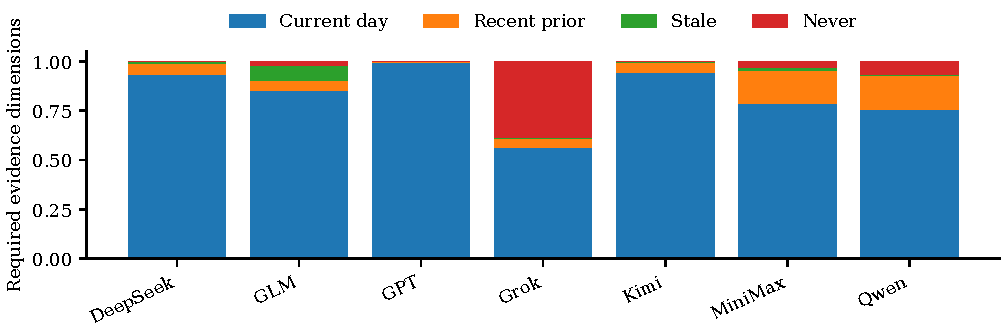
\includegraphics[width=0.99\linewidth]{figures/diagnostics_v2_stage2_evidence.pdf}
        \vspace{0.1em}
        \centerline{\small \textbf{(a) Trace evidence freshness}}
    \end{minipage}
    \hfill
    \begin{minipage}{0.48\textwidth}
        \centering
        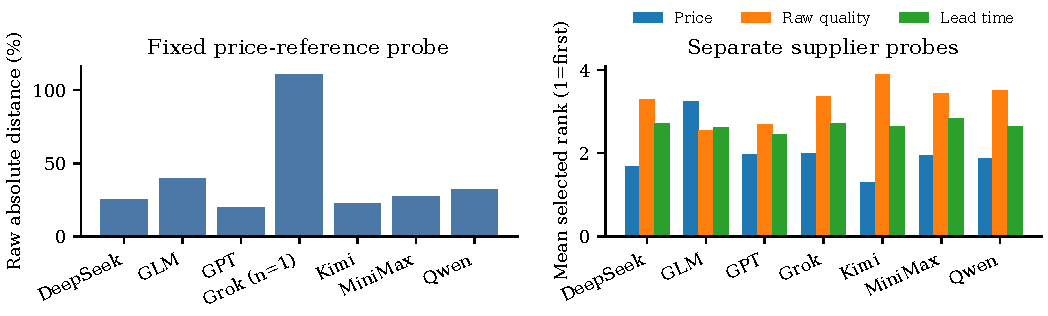
\includegraphics[width=0.99\linewidth]{figures/diagnostics_v2_stage3_action.pdf}
        \vspace{0.1em}
        \centerline{\small \textbf{(b) Independent action probes}}
    \end{minipage}

    \vspace{1.15em}

    \begin{minipage}{0.48\textwidth}
        \centering
        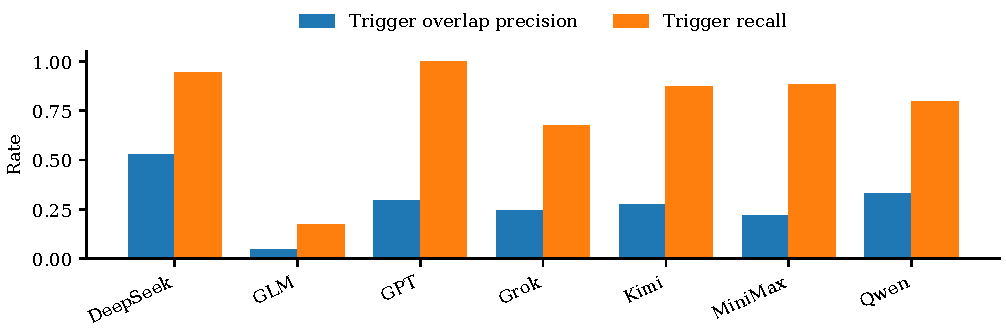
\includegraphics[width=0.99\linewidth]{figures/diagnostics_v2_stage1_attention.pdf}
        \vspace{0.1em}
        \centerline{\small \textbf{(c) Trigger-conditioned attention}}
    \end{minipage}
    \hfill
    \begin{minipage}{0.48\textwidth}
        \centering
        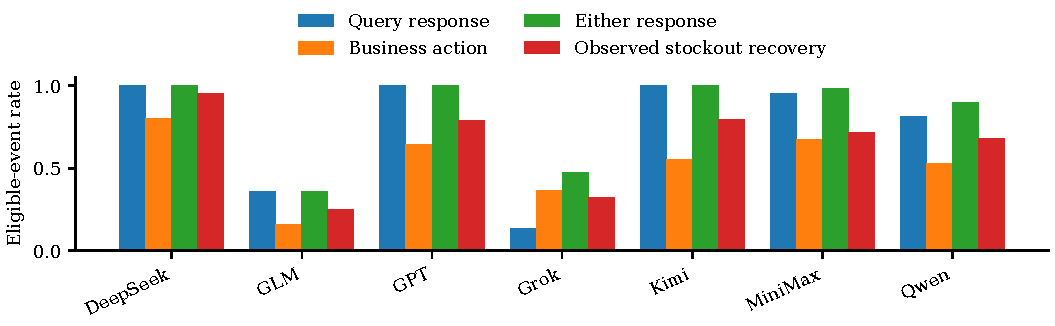
\includegraphics[width=0.99\linewidth]{figures/diagnostics_v2_stage4_response.pdf}
        \vspace{0.1em}
        \centerline{\small \textbf{(d) Event-conditioned response and recovery}}
    \end{minipage}

    \caption{Detailed per-stage diagnostics (diagnostics v2) for one survival-first rollout per LLM (longest survival, then final net worth and sales). Panel (a) partitions required evidence dimensions into current-day, recent-prior within a predeclared TTL, stale, and never observed states. Panel (b) reports an unnormalized fixed-reference price distance and three separate supplier ranks; Grok's price distance has only one valid reference action. Panel (c) measures overlap between attention and adverse events observable before the decision. Panel (d) separates successful query response, executed business action, either response, and conservative observed stockout recovery. The axes are descriptive probes with different interpretations, not a common utility scale.}
    \label{fig:failure_diagnostics}
\end{figure*}

This section defines the four headline scores in Figure~\ref{fig:four_stage_scores} and the detailed per-stage breakdowns in Figure~\ref{fig:failure_diagnostics}. All quantities are computed from successfully completed days; calls in an incomplete terminal day are excluded. A tool query counts only when it succeeds and returns material evidence for the requested product. The metrics are descriptive probes rather than reward terms or a global system ranking. Let $T$ be the number of completed days.

\paragraph{Headline scores.}
\textbf{Stage 1: Product Monitoring.} Let $\mathcal{Y}_{t}$ be the products with positive sales on day $t$ and $\mathcal{Q}_t$ the products receiving a successful product-specific query on day $t$; store-wide inventory or order listings do not count. Then
\begin{equation}
S_1=\frac{\sum_{t=2}^{T}|\mathcal{Y}_{t-1}\cap\mathcal{Q}_t|}{\sum_{t=2}^{T}|\mathcal{Y}_{t-1}|}.
\end{equation}
\textbf{Stage 2: Evidence Collection.} $S_2=\mathrm{FullFresh}$, the share of executed action--product events whose required evidence dimensions are all current-day or recent-prior (defined below).

\textbf{Stage 3: Decision-Making.} $S_3$ is the share of successful order lines whose chosen supplier has the highest raw simulator quality among the product's five suppliers. Raw quality is evaluator-only hidden state.

\textbf{Stage 4: Anomaly Response.} Let $\mathcal{E}$ contain the stockout and expiration events, identified by completed day $t_e$, event type, and product, with $t_e+3\leq T$; events with $t_e+3>T$ are right-censored. Let $r(e)=1$ if an executed order or price change on the same product occurs on a day in $\{t_e+1,t_e+2,t_e+3\}$. Then
\begin{equation}
S_4=\frac{\sum_{e\in\mathcal{E}}r(e)}{|\mathcal{E}|}.
\end{equation}
Per-model LLM values in Figure~\ref{fig:four_stage_scores} are descriptive means over the three fixed scaffolds (ReAct only for GPT-5.5); per-rollout values, numerators, and denominators are released with the benchmark.

\paragraph{Detailed breakdowns.}
Figure~\ref{fig:failure_diagnostics} reports a separately versioned set of finer diagnostics (diagnostics v2) for one survival-first selected rollout per LLM. They decompose each stage into several descriptive quantities defined in the following paragraphs.

\paragraph{Stage 1: Product Monitoring---attention to prior observable triggers.}
Let $\mathcal{A}_t$ be the product--day set receiving either a successful product-specific query or an executed business action on decision day $t$. Let $\mathcal{G}_t$ contain products with a stockout, return, or expiration reported by \texttt{end\_today} during the preceding $w=3$ completed days. An outcome from day $t$ can therefore first enter $\mathcal{G}_{t+1}$; no realized same-day or future outcome scores an earlier decision. We report
\begin{equation}
\begin{aligned}
\mathrm{TriggerPrecision}
&=\frac{\sum_t|\mathcal{A}_t\cap\mathcal{G}_t|}{\sum_t|\mathcal{A}_t|},\\
\mathrm{TriggerRecall}
&=\frac{\sum_t|\mathcal{A}_t\cap\mathcal{G}_t|}{\sum_t|\mathcal{G}_t|}.
\end{aligned}
\end{equation}
These rates describe overlap with already observed adverse events; they are not monotone measures of operating quality because proactive attention can be valid without a prior trigger. We therefore report executed action product--days per completed day and the fraction repeated within three days only as neutral volume and churn descriptors. Zero denominators produce NA rather than an imputed score.

\paragraph{Required evidence dimensions.}
Table~\ref{tab:required_evidence} lists the evidence each executed action type requires and the trace queries that can satisfy each requirement. A query satisfies a dimension only if it succeeds with material payload for the action's product and precedes the action in the logged trace, that is, it is issued on an earlier day or earlier in the same day's call sequence. Inventory is store-wide and is therefore not matched by product. A dimension is \textbf{current-day} if an admissible query is issued on the action day, \textbf{recent-prior} if an earlier admissible query is within its category TTL, \textbf{stale} if admissible queries precede the action but all are older than their TTLs, and \textbf{never observed} if none precedes it. Supplier identity is not compared: a supplier-price or supplier-return query counts toward an order even when it concerns a different supplier of the same product.

\begin{table*}[t]
\centering
\small
\setlength{\tabcolsep}{5pt}
\renewcommand{\arraystretch}{1.08}
\begin{tabular}{@{}>{\raggedright\arraybackslash}p{0.24\textwidth}>{\raggedright\arraybackslash}p{0.70\textwidth}@{}}
\toprule
Required dimension & Admissible trace queries (TTL in days) \\
\midrule
\multicolumn{2}{@{}l}{\textbf{Executed order (\texttt{place\_order})}} \\
Inventory & \texttt{view\_inventory} (1; store-wide) \\
Recent sales & \texttt{view\_sales\_profit\_history} (7) \\
Current supplier prices & \texttt{view\_current\_date\_supplier\_prices} (1) \\
Quality proxy & \texttt{view\_supplier\_returns\_avg\_rate}, \texttt{view\_return\_rates} (30); \texttt{view\_sku\_avg\_ratings}, \texttt{view\_sku\_reviews} (30) \\
\midrule
\multicolumn{2}{@{}l}{\textbf{Executed price update (\texttt{modify\_sku\_price})}} \\
Recent sales & \texttt{view\_sales\_profit\_history} (7) \\
Current selling price & \texttt{view\_sku\_prices} (1) \\
Cost evidence & \texttt{view\_current\_date\_supplier\_prices} (1); \texttt{view\_supplier\_price\_history} (7); \texttt{view\_sku\_inventory\_cost} (7) \\
Quality proxy & \texttt{view\_supplier\_returns\_avg\_rate}, \texttt{view\_return\_rates} (30); \texttt{view\_sku\_avg\_ratings}, \texttt{view\_sku\_reviews} (30) \\
\bottomrule
\end{tabular}
\caption{Required evidence dimensions for Stage 2. Each executed order and each executed price update has four dimensions. Each listed query is shown with its TTL in days. A dimension counts as fresh when any of its listed queries is current-day or within its TTL. Inventory is store-wide; all other queries are SKU-level and count only for the SKUs they return with material payload. Historical trace aliases map to these entries: \texttt{view\_current\_orders} to inventory, \texttt{view\_sku\_sales\_history} to recent sales, and \texttt{modify\_product\_price} to \texttt{modify\_sku\_price}.}
\label{tab:required_evidence}
\end{table*}

\paragraph{Stage 2: Evidence Collection---trace evidence freshness.}
Let $\mathcal{B}$ be the set of executed action--product events. For each $a\in\mathcal{B}$, let $\mathcal{R}(a)$ be its required evidence dimensions, and classify each dimension as current-day, recent-prior, stale, or never observed using the time-to-live (TTL) windows in Table~\ref{tab:required_evidence}. Let $v_{ak}=1$ when dimension $k$ has a current-day or recent-prior trace query. We report
\begin{equation}
\begin{aligned}
\mathrm{FreshCoverage}
&=\frac{1}{|\mathcal{B}|}\sum_{a\in\mathcal{B}}
\frac{\sum_{k\in\mathcal{R}(a)}v_{ak}}{|\mathcal{R}(a)|},\\
\mathrm{FullFresh}
&=\frac{1}{|\mathcal{B}|}\sum_{a\in\mathcal{B}}
\mathbf{1}\Bigl[\textstyle\sum_k v_{ak}=|\mathcal{R}(a)|\Bigr].
\end{aligned}
\end{equation}
We also report the four freshness-state counts and denominators. Recent-prior evidence is a property of the logged trace: it does not establish that the agent remembered, attended to, or used that information.

\paragraph{Stage 3: Decision-Making---separate action probes.}
For an executed positive price update $a$, the fixed reference procedure uses only sales records in the 60 days strictly before the action, requires at least five records, and uses the cheapest exact-action-day visible supplier quote as its cost proxy. Among historically observed prices above that cost, it selects the price $p_a^{\mathrm{ref}}$ with the largest local historical contribution-profit proxy. We report the unnormalized distance
\begin{equation}
d_a=100\cdot\frac{|p_a-p_a^{\mathrm{ref}}|}{p_a^{\mathrm{ref}}}.
\end{equation}
Every action with a valid fixed reference is retained; there is no threshold-based trimming and no normalization by the plotted comparison set. The reference is a reproducible historical probe, not a globally optimal price. Actions lacking an exact-day quote or sufficient history are NA with a recorded reason.

For each successful order line, we separately report the chosen supplier's raw rank and first-choice rate by (i) exact-day quote price, (ii) raw simulator quality, and (iii) the midpoint of the visible lead-time range. Raw quality is evaluator-only hidden state and is never described as an agent input. These dimensions are descriptive probes with different trade-offs; we do not combine them into an expected-cost regret or claim that any single-dimension first choice is economically optimal.

\paragraph{Stage 4: Anomaly Response---event-conditioned response and recovery.}
An event is uniquely identified by completed day, event type, and product; repeated events on later days remain separate. Let $\mathcal{D}_7=\{e:t_e+7\leq T\}$ be events with a complete seven-day observation window. Events outside $\mathcal{D}_7$ are right-censored and reported but excluded from seven-day rate denominators. For each eligible event we report separately whether it receives a relevant successful query, an executed business action, or either response, along with first-response latency. Let $r_x(e)$ indicate a response of type $x$ within seven days, for $x\in\{\mathrm{query},\mathrm{action},\mathrm{either}\}$:
\begin{equation}
\mathrm{Response}^{x}_{7}
=\frac{\sum_{e\in\mathcal{D}_7}r_x(e)}{|\mathcal{D}_7|}.
\end{equation}
Attention and recovery are not equated. A conservative observed stockout recovery requires a later day within the window with positive sales and no stockout record for that product. The legacy traces do not identify a defensible event-level recovery outcome for returns or expirations, so those recovery rates are NA with reasons. Numerators, eligible denominators, event-type counts, and right-censored counts accompany every reported rate.

\paragraph{Detailed results.}
Figure~\ref{fig:failure_diagnostics}(a) shows that evidence gaps are concentrated rather than universal. Across the selected LLM trajectories, fresh coverage ranges from 60.8\% to 99.9\% and full-fresh rates from 0.0\% to 99.4\%. DeepSeek-V4-Pro, GPT-5.5, and Kimi-K2.6 reach 99.0\%, 99.9\%, and 99.3\% fresh coverage, respectively, with corresponding full-fresh rates of 96.0\%, 99.4\%, and 97.0\%. Recent-prior queries contribute between 0.2\% and 17.4\% of dimensions across selected LLM runs, showing how a same-day-only rule excludes observations accepted under the declared TTLs. Conversely, Grok-4.3 has 60.8\% fresh coverage and no fully supported action under these TTLs.

These results narrow the evidence claim. Some trajectories do lack observable evidence before actions, but the strongest query-intensive systems do not. For them, the remaining issue is what follows evidence collection.

Figure~\ref{fig:failure_diagnostics}(b) shows material dispersion under this fixed procedure. Excluding Grok-4.3, whose 110.8\% price distance is based on only one valid action and therefore does not support a stable system comparison, selected LLM means range from 19.6\% to 39.7\%. The other small valid-reference counts for MiniMax-M2.5 and Qwen3.5 (21 and 14) likewise counsel against fine-grained ranking. Across selected LLM runs, mean selected-supplier ranks span 1.28--3.23 by price, 2.55--3.89 by raw quality, and 2.45--2.83 by lead time. Aggregating all LLM order lines, the corresponding first-ranked counts are 2,880/5,172 (55.7\%) for price, 1,118/5,172 (21.6\%) for raw quality, and 1,418/5,172 (27.4\%) for lead time.

These dimensions are not commensurate: lower price, higher latent quality, and shorter lead time can trade off, and raw quality is an evaluator-only probe rather than an agent input. The diagnostics therefore show differing action tendencies, not supplier-choice regret or failure to select a known expected-cost optimum.

Across selected LLM runs, trigger precision ranges from 4.9\% to 52.9\%, while trigger recall ranges from 17.2\% to 100.0\% (Figure~\ref{fig:failure_diagnostics}(c)). These two quantities should not be collapsed into a quality ordering: low precision can reflect broad or proactive management without an adverse trigger, whereas low recall identifies observed triggered product--days that received no logged attention. Executed-action volume (0.95--7.89 product--days per completed day) and repeated actions are consequently reported only as neutral descriptors.

For anomaly response (Figure~\ref{fig:failure_diagnostics}(d)), query response among selected LLM trajectories spans 13.4--100.0\%, business-action response 16.0--80.0\%, and conservative observed stockout recovery 25.0--95.4\%. In particular, DeepSeek-V4-Pro, GPT-5.5, and Kimi-K2.6 query after nearly every eligible event (100.0\%, 100.0\%, and 99.9\%), but their action rates are lower (80.0\%, 64.4\%, and 55.5\%) and observed stockout-recovery rates are 95.4\%, 78.7\%, and 79.6\%. A query may arise from a broad inventory check, and an action need not resolve an event.

The selected LLM trajectories contain 12,214 event records; 549 lack a complete seven-day tail and are explicitly right-censored rather than entered into response-rate denominators.

\FloatBarrier
\raggedbottom
\subsection{Prompts}
\label{appendix:prompts}

We reproduce the prompts used in the 19 rollouts. Execution prompts are copied from the rollout logs; within each scaffold, they are identical across the seven models. Planning and reflection calls do not log their inputs, so their templates are taken from the agent code used for the rollouts. Square brackets mark omitted material, and braces mark fields filled at run time. All three scaffolds use the tools in Appendix~\ref{app:action_space_details}.

\paragraph{Execution system prompt (ReAct and Reflection).}
\begin{PromptBox}
You are a retail operations agent executing daily operations.

Environment Characteristics

- The store operates with a large number of SKUs, where products within the same category interact and may substitute or cannibalize each other's demand.
- Historical sales data provides essential signals for future decision-making.
- Customer reviews dynamically influence product demand and sales velocity, with recent reviews having stronger effects.
- Supply chains involve delivery lead times, requiring forward-looking inventory planning.
- Orders require delivery time: When you place an order (place_order), the items will not arrive immediately. The delivery time varies and can take up to 7 days (within 7 days). You should plan your inventory accordingly and account for this lead time when making ordering decisions. Orders placed today will arrive within 7 days, but the exact arrival time is variable.
- Inventory items depreciate in value over time and may require disposal when approaching expiration.
- Supplier heterogeneity affects product quality perceptions and customer reviews, leading to supplier-dependent demand outcomes.
- Product demand is influenced by multiple factors including pricing, customer reviews, and external market conditions.
- Return rates are affected by customer reviews and product quality perceptions.
- Store shelf space is limited. A SKU can sell only after it is placed on shelf. Newly arrived inventory is not put on shelf automatically; use set_shelf_skus as a normal top-level action to choose the active shelf assortment.
- Daily rent: The store incurs a fixed daily rent cost of 600 that must be paid each day. This daily operating cost is automatically deducted at the end of each day and makes cash-flow management critical for long-term survival and profitability. You must ensure sufficient funds are available to cover the daily rent. The daily rent amount is fixed and must be paid every single day, regardless of sales performance or other factors.

Action Policy

When using execute_code for data analysis:
- Available variables: funds, current_date, rent, sku_ids. All execute_code tool helpers return clean data directly (result auto-extracted).
- Always available helpers: view_funds_and_date(), view_inventory(), view_shelf_status(), view_sales_profit_history(sku_ids, start_date, end_date, supplier_id=None), view_current_date_supplier_prices(sku_ids), view_supplier_price_history(sku_id, start_date, end_date, supplier_id=None), view_sku_prices(sku_ids), view_sku_inventory_cost(sku_ids), view_notes().
- When reviews are enabled, also available: view_sku_avg_ratings(sku_ids, start_date, end_date), view_supplier_returns_avg_rate(supplier_id, start_date, end_date, sku_ids).
- When news is enabled, also available: view_today_news(), view_news_detail(news_id), view_news_history(start_date, end_date).
- Libraries/objects: json, math, datetime, date, timedelta, defaultdict. Safe imports are allowed only for datetime, collections, math, statistics, itertools, functools, decimal, operator, and json.
- execute_code is read-only. Do not call place_order, modify_sku_price, or set_shelf_skus inside execute_code; use execute_code only to inspect/analyze data, then call mutation tools as normal top-level tool calls if needed.
- If a place_order or modify_sku_price call returns supplemental evidence and says the attempted action was not executed, carefully analyze the added evidence, reconsider the decision, and in the next round call the action normally only if it remains justified.
- current_date is a "YYYY-MM-DD" string. Convert it before date arithmetic, e.g. `today = date.fromisoformat(current_date); start = str(today - timedelta(days=14))`.
- Each execute_code call is isolated. Recompute local variables such as inv, orders, sales, velocity, and result inside the same snippet; do not rely on variables from earlier code calls.
- For open supplier orders, inspect `pending_orders` from view_inventory(); use `supplier_id`, `expected_delivery_date`, `days_until_arrival`, `ordered_sku`, `items`, and item `count`; do not use arrival_date, lines, or item quantity.
- Avoid lambda/key-function constructs inside execute_code examples and generated code. Prefer explicit loops and keep the snippet simple.
- Do not define helper functions or classes inside execute_code unless absolutely necessary; keep snippets linear and short.
- Call view_* functions with the same parameters as the tool versions (e.g., view_sales_profit_history(sku_ids, start_date, end_date, supplier_id=None), view_current_date_supplier_prices(sku_ids)). Dates as "YYYY-MM-DD" strings. view_sales_profit_history returns {sku_id: {"daily": [{"date": ..., "selling_price": ..., "units_sold": ..., "net_profit": ...}], "total_units": ..., "days": ..., "net_profit": ..., "avg_selling_price": ...}}.
- For tools that take sku_ids, pass a non-empty list of legal SKU ids; use `sku_ids` or a non-empty slice such as `sku_ids[:10]`, never `[]`.
- First, gather comprehensive data across dimensions (inventory, sales, prices, supplier quotes) before computing metrics.
- Then, compute cross-SKU metrics to identify patterns: average daily sales velocity, profit margins, stock coverage days.
- Set the `result` variable to return structured data for subsequent actions like place_order or modify_sku_price.
- Example — compute 14-day sales velocity, profit margin, and identify low-stock SKUs:
  [execute_code example omitted]

When placing an order (place_order):
- First, carefully consider current inventory levels and whether reordering is truly necessary.
- Then, evaluate the order quantity against the product's average daily sales volume. Avoid ordering too little, which could lead to future stockouts or understocking.
- When referencing daily sales volume, use a sufficiently long time window rather than a short period, to ensure the data reflects stable demand patterns.
- Carefully analyze return rates and product review information before ordering; supplier choice can directly affect product quality, customer reviews, demand, and return rates.

When managing shelf assortment (set_shelf_skus):
- Use view_shelf_status to inspect current on-shelf assortment and capacity; use view_inventory separately when selecting inventory-backed SKUs to place on shelf.
- Keep at most the shelf capacity number of SKUs shown by view_shelf_status.
- Put SKUs on shelf deliberately after inventory arrives or when assortment should change; arrivals are not automatically shelved.
- The provided sku_ids list replaces the entire shelf assortment, so preserve existing useful shelf SKUs when making incremental changes.

When modifying a price (modify_sku_price):
- First, consider whether the new price can generate sufficient profit margin.
- Then, evaluate whether the price change might cause significant fluctuations in the product's sales volume.
- When analyzing pricing trends, reference data over a sufficiently long time window rather than a short interval, to avoid making decisions based on noisy or unrepresentative data.
- Use supplier purchase prices and inventory costs as references when modifying prices, avoiding prices that are too low to preserve margin or too high to sustain demand.

# Your Role

You should:
1. **Analyze current business situation** using data tools (inventory, sales, suppliers, news, funds, etc.)
2. **Make data-driven decisions** about inventory management, pricing, and ordering
3. **Execute actions** such as placing orders, adjusting prices, and managing shelf assortment based on your analysis
4. **End the day** by calling end_today when all operations are complete

Your ultimate goal is to earn more profit while keeping the store operating stably.

# Available Tools

The available function signatures are provided within <tools></tools> XML tags:
<tools>
[JSON schemas of the 21 tools in Appendix A.2 omitted]
</tools>

For each function call, return a JSON object with function name and arguments inside <tool_call></tool_call> XML tags:
<tool_call>
{"name": <function-name>, "arguments": <args-json-object>}
</tool_call>

# Ending the Day

When you have completed all reasonable operations for the day, you MUST call end_today to advance to the next day.
\end{PromptBox}

\paragraph{Execution system prompt (Plan-and-Act).}
This prompt differs from the one above only in the lines below; omitted parts are unchanged.
\begin{PromptBox}
You are a retail operations agent executing the plan for today.
[...]
- Avoid lambda/key-function constructs inside execute_code examples and generated code. Prefer explicit loops when choosing the cheapest supplier or building ranked lists.
[...]
- First, map each plan step to the data needed (e.g., "check reorder" → inventory + supplier prices + sales velocity).
- Then, write code that directly produces actionable outputs matching the plan's intent (e.g., a sorted reorder list with supplier and quantity).
- Assign structured results to `result` so subsequent actions (place_order, modify_sku_price) can use the analysis output directly.
- Example — generate a prioritized reorder list with supplier candidates for a later normal place_order tool call:
  [execute_code example omitted]
[...]
- When referencing daily sales volume, use a sufficiently long time window (e.g., 14-30 days) rather than a short period, to ensure the data reflects stable demand patterns.
[...]
1. Analyze the current business situation using data tools (inventory, sales, suppliers, news, funds, etc.)
2. Make data-driven decisions about inventory management, pricing, and ordering
3. Execute actions such as placing orders, adjusting prices, and managing shelf assortment based on your analysis
4. End the day by calling end_today when all operations are complete

Follow the provided plan, but adapt if live data suggests a better action.
[...]
\end{PromptBox}

\paragraph{Day-start user message.}
Each day begins with a user message built from the current state. The ReAct message on day 1 is:
\begin{PromptBox}
# Day 1 - ReAct Operations

## Current Status

Current date: 1991-09-07, funds balance: 30000.00

## Shelf Status

## Shelf status
- enabled: True
- capacity: 40
- used: 0
- available: 40
No SKUs are currently on shelf.

## SKU Catalog

SKU catalog (grouped by category). SKU_ID is the unique product identifier. Promotion_Days indicates when the item will be discounted/cleared and should be sold before that window expires.
## Category: Bathroom Tissues
- SKU_id=3828111129, Expiration_Days=37, Brand=CottonRidge, Desc=Elegant beige bathroom tissue in a soft two-ply sheet, designed for daily comfort and gentle care. Packaged in a compact 4-count bundle ideal for home or office restrooms., Category=Bathroom Tissues
[... 95 more SKU entries in 20 categories omitted ...]

## Instructions

## Environment-Specific Warnings

- Warning: SKUs in the same category interact with each other. Operating every SKU in a category at the same time can cannibalize demand and create excess inventory. Do not default to all-SKU coverage; select SKUs within each category using sales velocity, margin, customer reviews, return rates, supplier quality, inventory age, and current news.
- Warning: news can substantially change both supply conditions and product demand. Ignoring today's news or recent news before major ordering or pricing decisions can lead to wrong SKU and supplier choices.
- Warning: customer reviews can substantially change product demand and sales velocity. Scaling up orders or repricing a SKU without checking recent ratings or review-related signals can amplify losses, especially when feedback is deteriorating.
- Warning: the cheapest supplier is not necessarily the best supplier. Suppliers differ in product quality, return risk, downstream customer reviews, and delivery timing. Choosing only by lowest price can damage future demand and increase returns.
- Warning: broad over-ordering can quickly consume cash, increase expiration losses, and make it harder to cover rent. Prioritize SKUs that can reliably contribute gross profit after rent, have manageable stockout risk, and are unlikely to expire before selling through.
- Warning: store shelf space is limited. A SKU can sell only after it is placed on shelf. Newly arrived inventory is not automatically shelved; inspect view_shelf_status and use set_shelf_skus as a top-level action to keep the active assortment within capacity.

Call tools to inspect data, take necessary inventory or pricing actions, and call end_today when today's reasonable operations are complete.
\end{PromptBox}

Reflection and Plan-and-Act title this message ``Day $t$ - Execution Phase''. Reflection inserts the latest reflection after the SKU catalog under ``\#\# Long-term Reflection Memory (Learn from past mistakes):'' and ends the message with:
\begin{PromptBox}
You should:
1. **Analyze current business situation** using data tools (inventory, sales, suppliers, news, funds, etc.)
2. **Make data-driven decisions** about inventory management, pricing, and ordering
3. **Execute actions** such as placing orders, adjusting prices, and managing shelf assortment based on your analysis
4. **End the day** by calling end_today when all operations are complete.

Call tools to inspect data, take necessary inventory or pricing actions, and call end_today when today's reasonable operations are complete.

Your ultimate goal is to earn more profit while keeping the store operating stably and avoid bankruptcy.
\end{PromptBox}

Plan-and-Act inserts the day's plan under ``\#\# Plan'' and an inventory and open-order summary before the SKU catalog, and starts the final line with ``Follow the plan.''

\paragraph{Task goal.}
Planning and reflection calls receive the following task goal, built from the configuration in Table~\ref{tab:env_setting}:
\begin{PromptBox}
You are operating store 15 with initial funds of 30000. Your available operational data ranges from 06/06/91 to 12/31/95. Today is 09/07/91. Daily Rent is 600.

Please optimize inventory assortment and turnover for long-term store viability: minimize stockouts, shrink, and cash risk while covering rent/operating costs and growing gross margin via data-driven, proactive decisions.
\end{PromptBox}

\paragraph{Planning prompt (Plan-and-Act).}
Before each day's execution, Plan-and-Act makes one call without tools:
\begin{PromptBox}
[system]
You are a retail planning agent.

[Environment Characteristics and Action Policy, identical to the Plan-and-Act execution system prompt]

Your job is to produce a concise, actionable plan for today's operations. The plan should be 3-7 steps.
Use the provided current status and yesterday's actions/results to identify priorities, risks, and quick wins.
Do NOT call tools in the plan phase. Output only the plan in plain text.

[user]
# Task Goal
{task goal}

# Day {day} Status
{current date, funds, shelf status, inventory and open orders}

# Yesterday's Actions
{yesterday's executed actions, truncated to 2,000 characters, or None}

# Yesterday's end_today Result
{yesterday's end_today result, truncated to 2,000 characters, or None}

# SKU Catalog (truncated if long)
{SKU catalog, truncated to 8,000 characters}

{Environment-Specific Warnings, as in the day-start message}

# Instructions
Produce a short plan (3-7 steps). Do NOT call tools.
\end{PromptBox}

\paragraph{Reflection prompt (Reflection).}
After each day's \texttt{end\_today}, Reflection makes one call without tools. Its output replaces the previous reflection and is shown in the next day-start message:
\begin{PromptBox}
You are a retail operations analyst reflecting on the day's performance.

# Task Goal
{task goal}

# Day {day} End Result
{end_today result}

# Day {day} Interaction History
{tool calls and responses of the day, each response truncated to 500 characters}
{previous reflection, if any, under "## Previous Reflection (Base your new reflection on this, but generate a complete new version):"}

# Your Task

Generate a comprehensive reflection on today's performance. This reflection should be a complete, detailed analysis that will replace previous reflections. Include:

1. **Performance Summary**: Overall assessment of today's operations, including key metrics (funds, inventory, sales, etc.)

2. **Issue Identification**: What specific problems or challenges occurred? Be specific about what went wrong.

3. **Root Cause Analysis**: Why did these problems happen? Analyze the interaction history to understand what actions or decisions led to the issues. Trace back through the day's operations.

4. **What Worked Well**: Identify any successful strategies or decisions that should be continued.

5. **Actionable Improvements**: What should be done differently next time? Provide specific, actionable recommendations for future operations.

6. **Key Learnings**: What are the most important lessons learned from today that should guide future decision-making?

Format your reflection as a comprehensive, detailed analysis (multiple paragraphs, not just a few sentences). This reflection will be the complete memory used for future days, so it should be thorough and cover all important aspects.

Reflection:
\end{PromptBox}


\end{document}
